\section{Introduction}
Chapter~\ref{ch:nmrf} and~\ref{ch:pseudo-label} introduced neural Markov random fields for stereo matching, a framework that recasts classical graphical-model inference as a learnable message-passing network.
The key advantage of this formulation is that it preserves an important geometric inductive bias of stereo vision: depth is inferred by selecting, propagating, and refining disparity hypotheses under local spatial consistency constraints.
By combing disparity proposal generation, neural message passing, and learned regularization, the resulting model achieves accurate and efficient stereo matching while retaining the interpretability of hypothesis-based correspondence reasoning.
Nevertheless, the approach remains fundamentally stereo-centric.
Its evidence comes primarily from correspondences between two views, and it therefore inherits a central limitation of stereo matching: when image correspondence becomes unreliable, the recovered geometry may also become unstable as well.

This limitation is closely connected to the broader motivation of this thesis.
Robust visual geometry is difficult to recover from a single source of evidence.
Stereo correspondence provides metric constraints through epipolar geometry and is highly effective when reliable matches are available.
Yet stereo reasoning is fragile in regions where matching is ambiguous or misleading, including weakly textured surfaces, repetitive patterns, occlusions, transparent materials, and specular reflections.
These failures are not merely artifacts of a particular network architecture.
They reveal an intrinsic weakness of correspondence-based geometry: when the image evidence does not uniquely identify the correct match, local matching alone cannot provide a stable geometric explanation.

Monocular perception provides a complementary form of evidence.
Although a single image cannot uniquely determine metric 3D structure, it contains rich contextual cues, including semantic layout, object-level regularities, perspective, surface continuity, and learned priors about scene organization.
Recent large-scale monocular foundation models~\cite{ranftl2020towards,ke2023repurposing,depth_anything_v1,piccinelli2024unidepth} have substantially strengthened this form of holistic depth reasoning, producing coherent depth ordering and plausible scene  structures across diverse visual domains.
Such models can be more robust than stereo matching in regions where local correspondence is ambiguous, because they can infer structure from global context rather than relying only on pixel-level matching evidence.
At the same time, monocular depth remains geometrically under-constrained.
Without explicit multi-view constraints, monocular predictions may lack metric accuracy, fine local details, and reliable scale.

The natural step beyond neural MRF stereo matching is therefore not to abandon correspondence reasoning, but to enrich it with monocular context while preserving the metric precision of stereo geometry.
This chapter explores that direction by studying how monocular and stereo representations can be unified during geometrical reasoning.
The central observation is that their strengths are complementary at the level of latent representation.
Monocular features provide structural priors that can regularize ambiguous disparity hypotheses, while stereo hypotheses provide metric geometric evidence that can ground monocular depth reasoning.
A unified model should therefore allow these two forms of reasoning to interact before the final prediction is made, rather than combining their outputs only after separate reasoning processes have already been completed.

To this end, this chapter presents \emph{BridgeDepth}, a latent alignment approach that integrates monocular contextual reasoning and stereo geometric matching within a single network.
Instead of treating monocular depth as an external prior, an auxiliary prediction, or a post-hoc fusion signal, BridgeDepth introduces monocular contextual representations directly into the stereo hypothesis aggregation.
The monocular branch extracts structural features from a pretrained depth foundation model, while the stereo branch maintains a compact set of disparity hypotheses at each pixel.
To make cross-modal interaction efficient, the stereo search space is first pruned into a small number of representative hypotheses, following the proposal-based reasoning introduced in NMRF~\cite{guan2024neural}.
This compact hypothesis representation provides a tractable interface for aligning monocular context with stereo geometry.

The core of BridgeDepth is an iterative bidirectional latent alignment mechanism.
At each alignment step, stereo hypotheses first perform a \emph{monocular-readout} operation, in which they attend to monocular contextual features through cross-attention.
This operation allows semantic and structural priors to guide correspondence reasoning before stereo cost aggregation, especially in ambiguous regions where local matching evidence is weak or deceptive.
The stereo hypotheses are then aggregated through neural message passing, which propagates geometric consistency across neighboring pixels and resolves competition among candidate disparities.
After aggregation, a reverse \emph{monocular-update} operation lets monocular features attend back to the refined stereo hypotheses.
In this direction, geometrically validated correspondence information is injected into the monocular representation, reducing its ambiguity and improving its consistency with metric scene structure.
Through iterative readout, aggregation, and update operations, monocular context and stereo geometry are progressively synchronized in a shared latent space.

This bidirectional alignment design is important for the thesis narrative because it moves beyond treating visual geometry as a collection of isolated estimation problems.
The previous chapters showed that stereo matching benefits from structured hypothesis reasoning, where disparity candidates are refined through learned message passing under spatial consistency.
However, the source of geometric evidence in that formulation is still largely restricted to binocular correspondence.
BridgeDepth extends this reasoning paradigm by introducing monocular scene understanding into the hypothesis aggregation process.
Each disparity hypothesis is therefore evaluated not only by local matching evidence, but also by contextual priors about scene layout, object structure, and surface continuity.
At the same time, the monocular representation is updated by aggregated stereo hypotheses, so its contextual features become grounded by metric geometric constraints rather than remaining purely prior-driven.

This mechanism is more than a fusion strategy for improving stereo depth estimation.
It represents a step forward the broader goal of this thesis: learning unified geometric representations in which complementary visual cues interact during reasoning.
Rather than concatenating monocular and stereo features or applying a final-stage correction to the stereo output, BridgeDepth establishes a recurrent exchange between contextual priors and geometric evidence.
Through this exchange, monocular reasoning becomes more geometrically constrained, while stereo reasoning becomes more robust to ambiguous correspondence.
The resulting formulation reflects the central hypothesis of this thesis: robust structure and motion estimation requires a coherent latent space in which multiple sources of visual geometry, including spatial correspondence, semantic context, and eventually temporal motion cues, can be jointly represented and refined.

Following this principle, BridgeDepth preserves separate task-specific predictions while allowing their underlying representations to interact.
The framework produces two outputs: a metric disparity map from the stereo stream and a relative depth map from the monocular stream.
The stereo output remains the primary source of geometrically accurate reconstruction, as it is directly constrained by binocular correspondences.
The monocular output, however, is not merely an auxiliary prediction used for additional supervision.
Since the monocular representation is repeatedly updated by aggregated stereo hypotheses, its prediction indicates whether metric geometric evidence has been successfully injected into the contextual stream.
The dual-output design therefore encourages bidirectional alignment during training and provides a direct way to examine its effect: stereo reasoning becomes more robust through monocular priors, while monocular reasoning becomes more consistent with multi-view geometry.

The effectiveness of this design is validated through extensive experiments.
On standard stereo benchmarks, BridgeDepth achieves competitive or state-of-the-art accuracy while maintaining efficient inference.
More importantly, it substantially improves zero-shot generalization from synthetic training data to real-world datasets such as Middlebury and ETH3D, where domain shift and correspondence ambiguity are particularly challenging.
Qualitative results in Figure~\ref{fig:tsear}, further show stronger robustness on reflective and transparent surfaces, where conventional stereo methods often produce fragmented or physically implausible disparities.
These results support the central argument of this chapter: monocular context and stereo geometry should not be treated as independent estimators whose outputs are fused after separate prediction, but as complementary representations that are aligned and refined during latent reasoning.

\begin{figure}[!t]
	\centering
	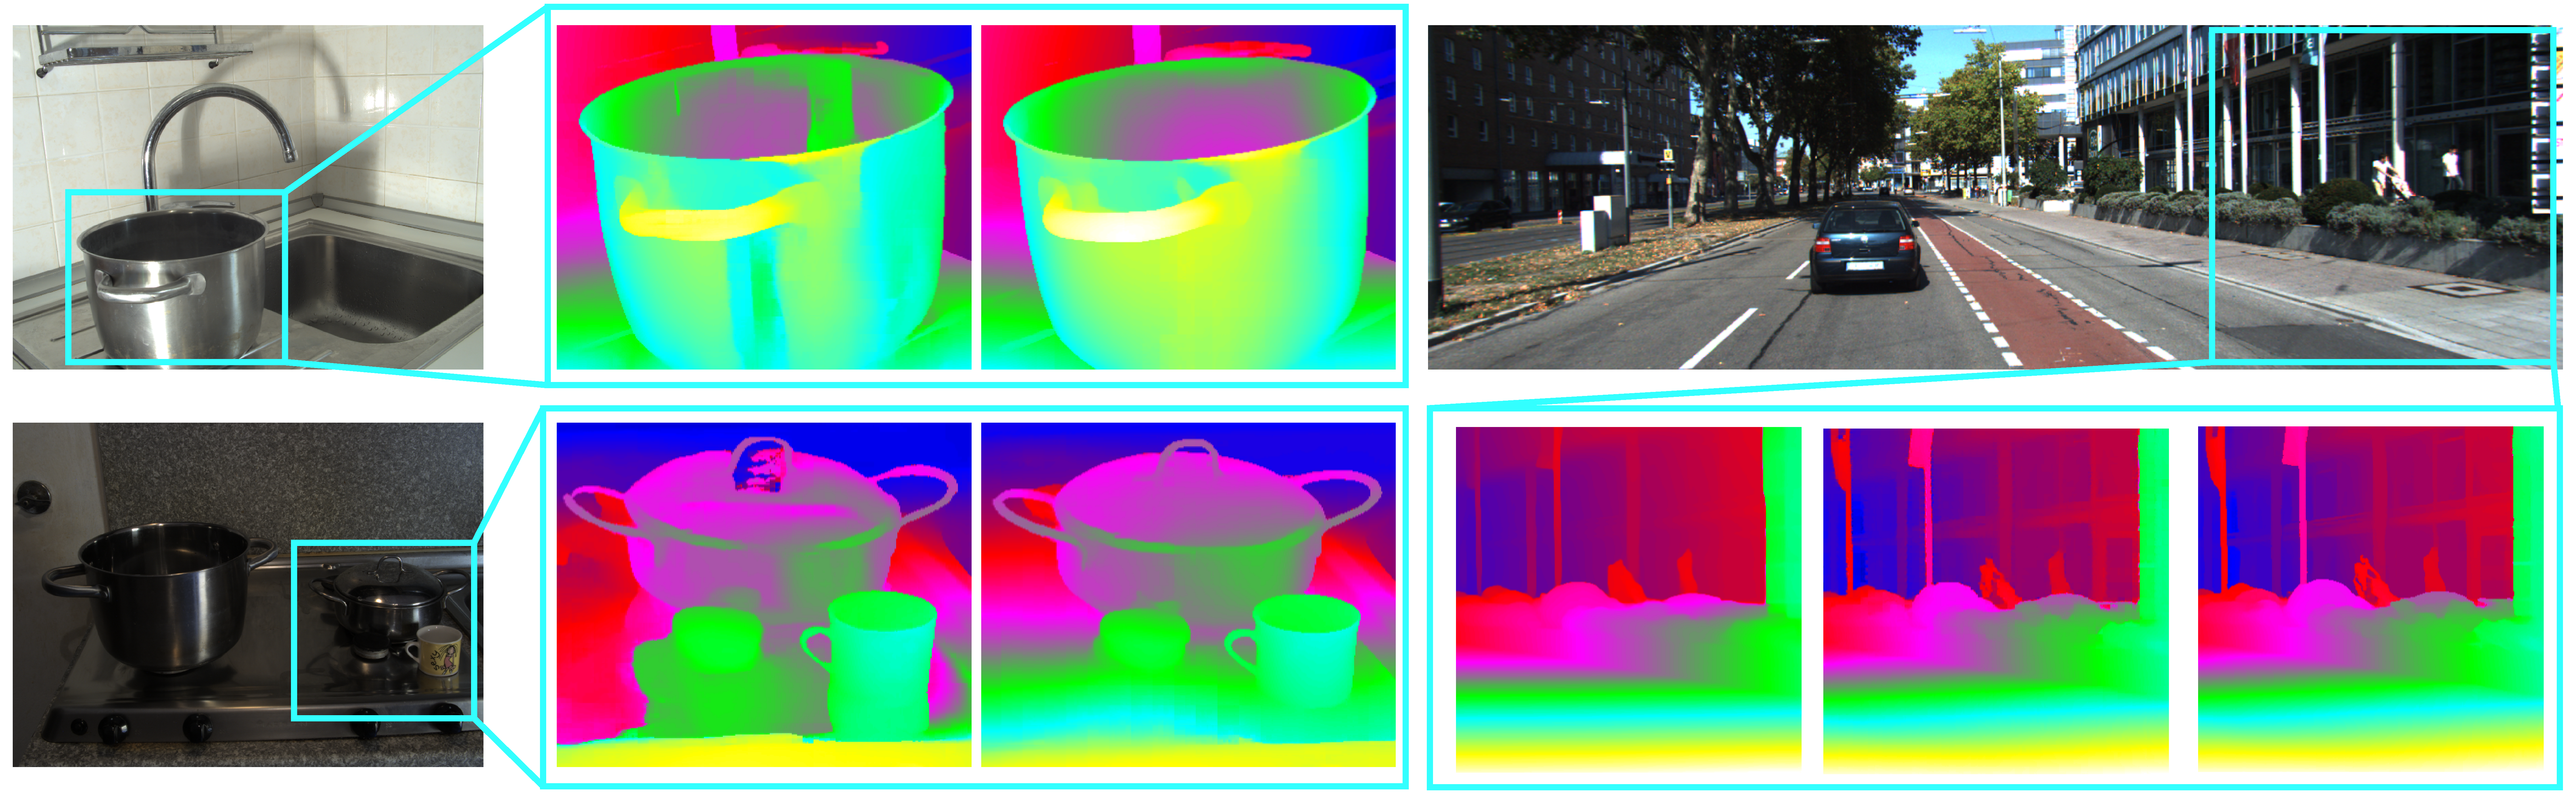
\includegraphics[width=0.99\linewidth]{fig/bridgedepth/bridgedepth.pdf}\\
	\makebox[0.21\linewidth]{}
	\makebox[0.16\linewidth]{\footnotesize \textsf{NMRF~\cite{guan2024neural}}}
	\makebox[0.17\linewidth]{\footnotesize \hspace{-0.5em}\textsf{Ours-\emph{Stereo}}}
	\makebox[0.14\linewidth]{\footnotesize \textsf{DepthAnythingV2~\cite{yang2024depth}}}
	\makebox[0.14\linewidth]{\footnotesize \textsf{Ours-\emph{Mono}}}
	\makebox[0.14\linewidth]{\footnotesize \textsf{Ours-\emph{Stereo}}}
	\vspace{-5pt}
	\captionof{figure}{By aligning latent representations, the proposed approach unifies monocular geometric reasoning with stereo matching.
	It achieves both higher overall depth accuracy and finer detail than the monocular baseline DepthAnythingV2~\cite{yang2024depth}, while also improving over the stereo method NMRF~\cite{guan2024neural}, particularly on textureless surfaces and reflective regions where correspondence is unreliable.}
	\label{fig:tsear}
	\vspace{-5pt}
\end{figure}

In summary, this chapter extends the hypothesis-based stereo architecture developed in Chapter~\ref{ch:nmrf} into a unified monocular and stereo reasoning formulation.
The proposed method preserves the metric precision of stereo matching while incorporating the robustness of monocular contextual reasoning.
By aligning spatial correspondence and semantic context within a shared representation, BridgeDepth provides a concrete instance of the broader thesis hypothesis: robust visual geometry emerges when complementary cues jointly shape the reasoning process rather than acting in isolation.

\section{Methodology}
\subsection{Overview of the Architecture}
Given a rectified stereo pair $\bm{I}_1, \bm{I}_2$, the approach estimates two outputs: a metric disparity map $D$ from the stereo reasoning stream and a relative depth map $R$ from the monocular reasoning stream.
The architecture consists of two stages, as illustrated in Figure~\ref{fig:bridgedepth_overview}.
The first stage, \textbf{pre-alignment}, constructs modality-specific representations.
The monocular stream processes the reference image $\bm{I}_1$ using a pretrained monocular depth foundation model and extracts a contextual feature map.
The stereo stream extracts multi-scale features from both images and uses a Disparity Proposal Network (DPN) to produce a small set of candidate disparities at each pixel.
Each candidate is then embedded as a latent stereo hypothesis.
The second stage, \textbf{bidirectional latent alignment}, iteratively synchronizes the monocular and stereo representations.
At each alignment step, stereo hypotheses first read from monocular features through cross-attention.
This readout injects contextual priors into the stereo hypotheses before cost aggregation.
The stereo hypotheses are then aggregated using neural message passing, which performs both inter-pixel propagation and intra-pixel hypothesis competition.
Finally, the monocular features are updated by attending to the aggregated stereo hypotheses, allowing geometrically validated information to flow back into the monocular stream.
A coarse-to-fine cascade further refines disparity at a higher spatial resolution.

This design differs from post-hoc fusion~\cite{bae2022multi,li2024local} in an important way. 
The monocular and stereo streams are not merely combined near the output.
Instead, they interact throughout the reasoning process, allowing the model to learn a shared latent space in which monocular context and stereo geometry mutually constrain each other.

\begin{figure}[!t]
	\centering
	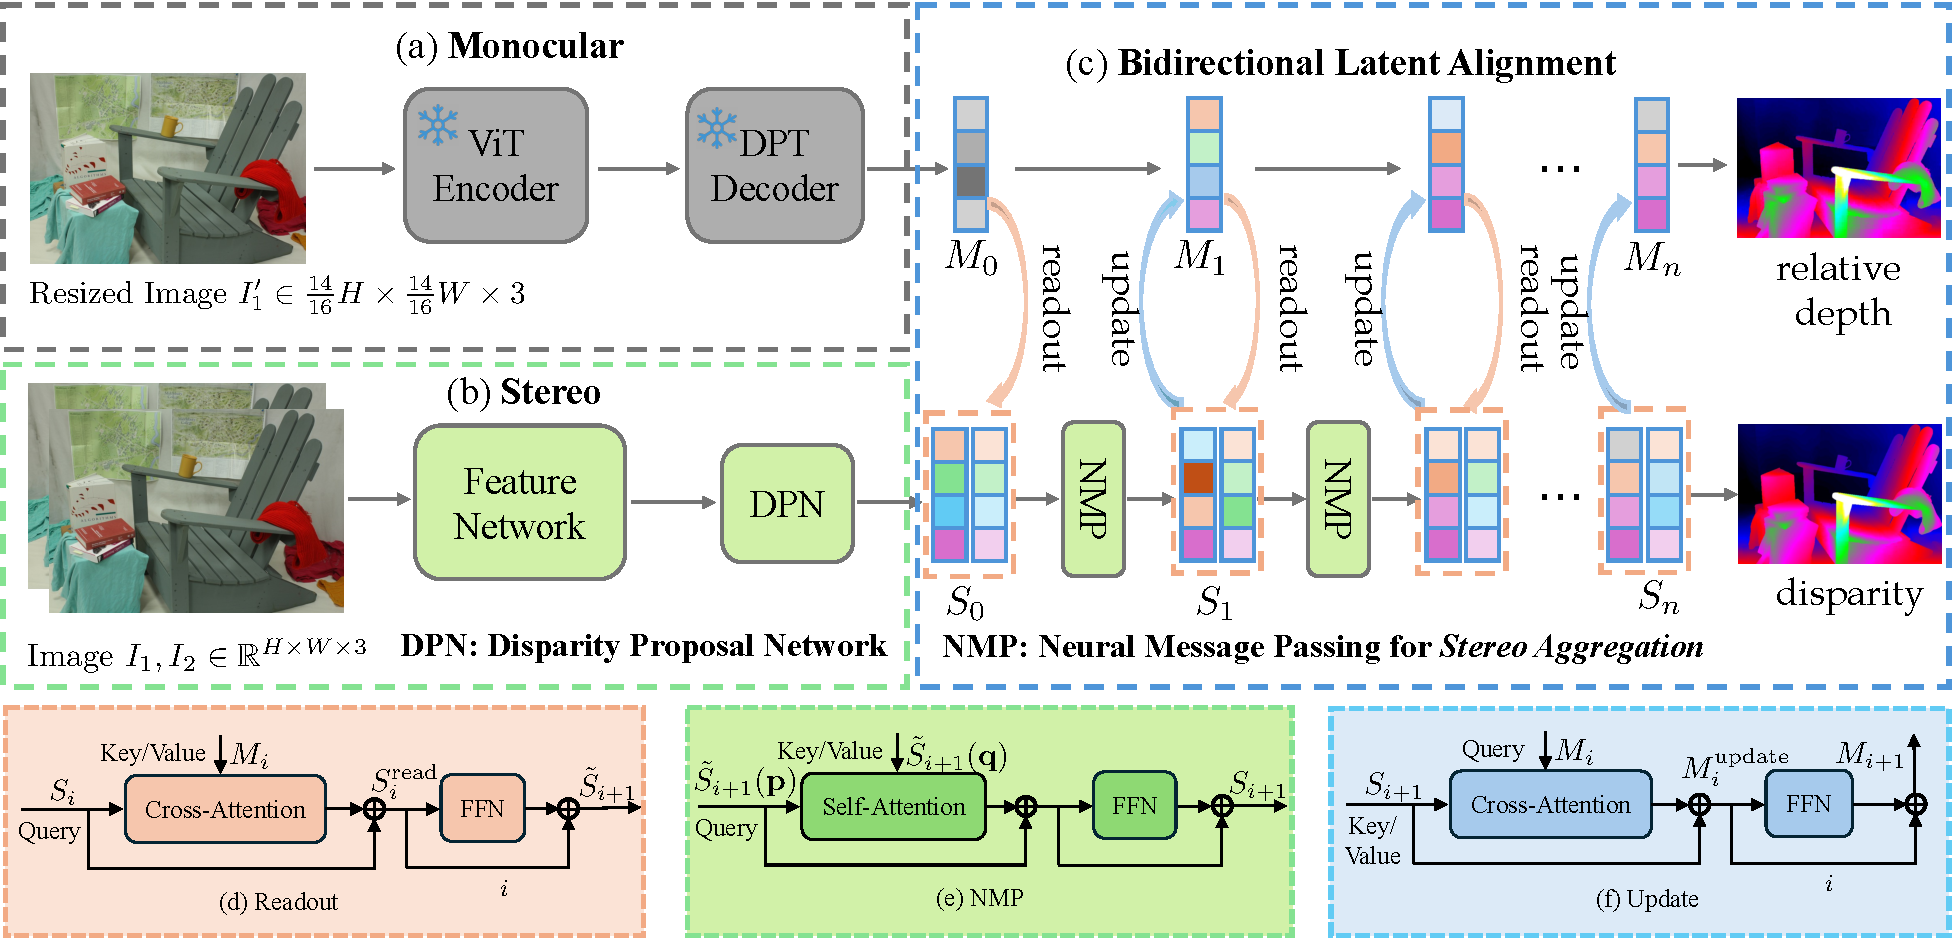
\includegraphics[width=0.97\linewidth]{fig/bridgedepth/bridgedepth_overview.pdf}
	\caption{\textbf{Architecture of the proposed BridgeDepth framework.} The model operates in two phases.
	During pre-alignment, (a) a monocular encoder aggregates contextual information from the reference view, while (b) a stereo pathway uses DPN~\cite{guan2024neural} to reduce the disparity search space from 40 labels to 2 candidate labels. 
	During bidirectional latent alignment, (c) the two modalities are iteratively synchronized through cross-modal interaction; spatial dimensions are collapsed in the diagram for clarity. 
	The network predicts relative depth from the monocular stream and metric disparity from the stereo stream.}
	\label{fig:bridgedepth_overview}
	\vspace{-0.8em}
\end{figure}

\subsection{Monocular Contextual Feature Extraction}
The monocular stream is initialized from a pretrained monocular depth foundation model.
In the implementation described in this chapter, the stream follows a  DepthAnything-style architecture that combines a DINOv2~\cite{oquab2023dinov2} visual encoder with a DPT~\cite{ranftl2021vision} decoder.
The pretrained encoder provides strong general-purpose visual features, while the decoder aggregates multi-level representations into dense contextual features for depth prediction.
Let $\bm{I}_1 \in \mathbb{R}^{H \times W \times 3}$ denote the reference image.
To match the $14\times 14$ patch size of the ViT encoder, the image is resized by a factor of $14/16$, producing $\bm{I}_1'$.
The DPT decoder outputs a feature map whose spatial resolution corresponds to $8/14$ of $\bm{I}_1'$, \ie one half of the original image resolution.
This feature map is then downsampled by a strided-4 convolution so that its resolution matches the coarse stereo branch.
The resulting monocular feature map is denoted as
$M_0 \in \mathbb{R}^{\frac{H}{8} \times \frac{W}{8} \times C}$.
The role of $M_0$ is not limited to monocular depth prediction. 
It serves as a contextual memory that encodes semantic layout, object structure, surface continuity, and monocular depth priors. 
These cues are later queried by stereo hypotheses during alignment.
In the main configuration, the pretrained monocular stream is frozen during training.
Freezing helps preserve the generalization capability learned from internet-scale data and prevents the stereo training set from over-specializing the monocular representation.
Additional experiments (see Table~\ref{tab:mono_foundation}) show that the framework is compatible with multiple monocular backbones, including diffferent variants of DepthAnythingV2~\cite{yang2024depth}, UniDepthV2~\cite{piccinelli2025unidepthv2}, and MoGe~\cite{wang2025moge,wang2025moge2} models.

\subsection{Stereo Hypothesis Representation}
\noindent\textbf{Multi-scale stereo feature extraction.}
The stereo stream extracts image features from the left and right views using a Siamese feature network.
For each scale $s \in \{4,8\}$, the network produces feature maps $\bm{F}_{1,s}, \bm{F}_{2,s} \in \mathbb{R}^{\frac{H}{s} \times \frac{W}{s} \times C}$, where $\bm{F}_{1,s}$ and $\bm{F}_{2,s}$ correspond to the reference and target images, respectively.
The $1/8$-resolution features are used for coarse stereo reasoning, while the $1/4$-resolution features are later used for fine-grained refinement.

A conventional cost-volume formulation would evaluate many disparity candidates at each pixel.
For example, if the maximum disparity is 320 pixels and the feature stride is 8, the coarse disparity dimension contains approximately 40 candidates.
Directly aligning such a dense cost volume with monocular features would be computationally expensive because cross-attention complexity grows quadratically with both the number of spatial tokens and the number of disparity hypotheses.

\noindent\textbf{Disparity hypotheses pruning.}
To make cross-modal alignment efficient, the stereo stream uses a disparity proposal mechanism to reduce the number of hypotheses.
Starting from the coarse feature maps $\bm{F}_{1,8}$ and $\bm{F}_{2,8}$, the proposal module computes matching scores over the initial disparity range and selects the top $K$ candidates for each pixel. 
In the default configuration, the full candidate set is reduced from 40 to $K=2$ hypotheses per pixel.
A disparity propagation module~\cite{guan2024neural} then refines the selected candidates by spreading plausible disparities over local neighborhoods and suppressing unlikely ones.
The resulting candidates are denoted by $\{d^k_{i,j}\}_{k=1}^{K}$,
where $d^k_{i,j}$ is the $k$-th disparity proposal at pixel $(i,j)$ on the coarse grid.
This compact representation preserves the main disparity modes while making bidirectional alignment tractable.

\noindent\textbf{Hypothesis embedding.}
Each disparity candidate is embedded into a latent vector that combines concatenation-based and correlation-based matching cues. For the $k$-th hypothesis at location $(i,j)$, the embedding is defined as
\begin{align}
	S_0(i,j,k)&=\text{FFN}\left(\mathbf{x}_{i,j,k}^{{\tt concat}} \parallel \mathbf{x}_{i,j,k}^{{\tt corr}}\right), \nonumber \\
	\mathbf{x}_{i,j,k}^{{\tt concat}}&=\delta_1\left(\bm{F}_{1,8}(i,j)\right) \parallel\delta_1\left(\bm{F}_{2,8}(i,j-d_{i,j}^{k})\right), \label{eq:hypothesis-embedding} \\
	\mathbf{x}_{i,j,k}^{{\tt corr}}(g)&=\frac{G}{C}\left\langle\delta_2(\bm{F}_{1,8}(i,j,g)),\delta_2(\bm{F}_{2,8}(i,j-d_{i,j}^k,g))\right\rangle \nonumber.
\end{align}
Here, $\parallel$ denotes channel concatenation.
The feature channels are divided into $G$ groups for grouped correlation, and $g$ indexes one group.
The functions $\delta_1$ and $\delta_2$ normalize the feature distributions before concatenation and correlation. 
Each consists of convolutional layers with normalization and nonlinear activation. 
For sub-pixel disparity proposals, bilinear sampling is used to obtain the right-image feature at the shifted location.
The embedded stereo hypotheses are collected as
$S_0 \in \mathbb{R}^{\frac{H}{8} \times \frac{W}{8} \times K \times C}$.
This tensor is the stereo counterpart of the monocular contextual features $M_0$ and serves as the input to the latent alignment module.

\subsection{Bidirectional Latent Alignment}
The bidirectional alignment module performs iterative interaction between monocular contextual features and stereo hypothesis embeddings.
Let $M_i$ and $S_i$ denote the monocular and stereo representations at iteration $i$.
Each iteration contains three operations: monocular readout, stereo aggregation, and monocular update.

\noindent\textbf{Monocular readout: context-guided stereo hypotheses.}
Before stereo aggregation, the stereo hypotheses query the monocular feature map, as illustrated in Figure~\ref{fig:bridgedepth_overview} (d).
This operation allows each disparity hypothesis to access contextual information such as object boundaries, semantic regions, and likely structure layout.
For efficiency, the feature maps are divided into non-overlapping $N\times N$ spatial windows.
Within each window, the stereo embeddings serve as queries, while the monocular features serves as key and values:
\begin{equation} \begin{aligned} Q_s = \mathrm{LN}(S_i) W_q, \quad K_m = \mathrm{LN}(M_i) W_k, \quad V_m = \mathrm{LN}(M_i) W_v. \end{aligned} \end{equation}
The readout operation is then defined as
\begin{align} 
	S_i^{\mathrm{read}} &= S_i + \mathrm{WindowAttn}(Q_s, K_m, V_m), \\ \widetilde{S}_{i+1} &= S_i^{\mathrm{read}} + \mathrm{FFN}\left(\mathrm{LN}(S_i^{\mathrm{read}})\right). 
	\label{eq:bridge_readout}
\end{align}
This produces contextual-aware stereo embeddings $\widetilde{S}_{i+1}$, which are subsequently aggregated by the stereo reasoning module.

\noindent\textbf{Content-adaptive positional bias.} The window attention in Equation~\ref{eq:bridge_readout} adopts a content-adaptive positional bias to preserve spatial structure during cross-modal interaction.
For query, key, and value tensors $Q$, $K$, and $V$, attention is computed as
\begin{equation} \mathrm{WindowAttn}(Q,K,V) = \mathrm{softmax}\left(\frac{QK^{\top}}{\sqrt{d}} + \beta \right)V, \end{equation}
with
\begin{equation} \beta = Q^{\top}R^k + K^{\top}R^q. \label{eq:bridge_pos_bias} \end{equation}
The learnable position embeddings $R^q$ and $R^k$ encode relative positions inside a window and distinguish the roles of query and key tokens.
Unlike a fixed relative bias, this formulation lets the positional term depend on feature content, allowing the attention mechanism to adapt spatial aggregation according to local image structure.

\noindent\textbf{Stereo aggregation by neural message passing.} After monocular readout, the stereo hypotheses are aggregated using neural message passing (NMP) module of NMRF, as depicted in Figure~\ref{fig:bridgedepth_overview} (e).
This module can be interpreted as a structured form of self-attention over the stereo hypothesis graph.
It performs two complementary operations.
First, inter-pixel aggregation propagates information between neighboring pixels.
This encourages adjacent pixels on the same surface to support consistent disparity hypotheses while still allowing discontinuities near object boundaries.
Second, intra-pixel aggregation models competition among multiple hypotheses at the same pixel.
This helps suppress inconsistent candidates and sharpen the posterior around the most plausible disparity.
The output of this aggregation step is denoted as
\begin{equation} S_{i+1} = \mathrm{NMP}\left(\widetilde{S}_{i+1}\right), \end{equation}
where $S_{i+1}$ contains stereo hypotheses that have been refined using both monocular contextual priors and geometric consistency from neighboring hypotheses.

\noindent\textbf{Monocular update: geometry-grounded contextual features.}
The second direction of alignment, shown in Figure~\ref{fig:bridgedepth_overview} (f), injects stereo-validated geometric information back into the monocular stream.
After stereo aggregation, the monocular features query the updated stereo embeddings:
\begin{equation} \begin{aligned} Q_m = \mathrm{LN}(M_i) W'q, \quad K_s = \mathrm{LN}(S_{i+1}) W'k, \quad V_s = \mathrm{LN}(S_{i+1}) W'_v. \end{aligned} \end{equation}
The monocular update is given by
\begin{align} 
	M_i^{\mathrm{update}} &= M_i + \mathrm{WindowAttn}(Q_m, K_s, V_s), \\
	 M_{i+1} &= M_i^{\mathrm{update}} + \mathrm{FFN}\left(\mathrm{LN}(M_i^{\mathrm{update}})\right).
	\label{eq:bridge_update} 
\end{align}
This operation grounds the monocular features with geometric evidence, including disparity boundaries, depth ordering, and local surface consistency.
The updated contextual representation is therefore no longer purely monocular; it becomes a geometry-aware latent representation refined by stereo geometry evidence.

\noindent\textbf{Iterative alignment.} The readout, aggregation, and update operations form one alignment block.
Stacking multiple blocks creates an iterative refinement process:
\begin{equation} (M_i, S_i) \rightarrow (M_{i+1}, S_{i+1}), \quad i=0,\ldots,l-1. \end{equation}
Each iteration improves the consistency between monocular and stereo representations.
Stereo hypotheses become more aware of global scene structure, while monocular features become more geometrically grounded.
This iterative exchange is the core difference between latent alignment and static feature fusion.

\subsection{Coarse-to-Fine Detail Recovery}
The main alignment stage operates at $1/8$ of input image resolution for efficiency.
Although this resolution is sufficient for robust global reasoning, it may miss thin structures and sharp disparity discontinuities.
To recover fine details, the model uses a coarse-to-fine refinement stage.
After $l$ iterations of coarse alignment, the stereo stream decodes a coarse disparity prediction $D_{\mathrm{coarse}}$. 
This disparity is downsampled to the $1/4$ scale using median pooling, which preserves discontinuities better than average pooling.
The downsampled disparity initializes a new set of fine-level stereo embeddings using the $1/4$-resolution image features $\bm{F}_{1,4}$ and $\bm{F}_{2,4}$.
The same feature-warping and grouped-correlation formulation used to construct $S_0$ is applied at this higher resolution.

To balance accuracy and efficiency, the stereo stream is refined at $1/4$ resolution while the monocular stream remains at $1/8$ resolution.
Since the two streams now have different spatial scales, the cross-attention window size of the monocular stream is adjusted so that windows in both stream cover an equivalent image region.
In practice, if the stereo window size is $N$, the monocular window size is reduced to $N/2$.
This asymmetric design allows the framework to recover fine geometric structures without running full monocular-stereo alignment at high resolution.
The fine-level stereo embeddings continue to query monocular context and update the monocular representation, while the computational cost remains manageable.

\subsection{Dual Output Prediction}
After the coarse and fine alignment stages, the model decodes two outputs: metric disparity from the stereo stream and relative depth from the monocular stream.
The stereo decoder maps the final stereo embeddings to a full-resolution disparity map.
A lightweight multilayer perceptron projects the $1/4$-resolution embeddings into a feature tensor with 16 channels for spatial reconstruction. 
A pixel shuffle operation then produces the full-resolution disparity map $D \in \mathbb{R}^{H \times W}$.
The monocular decoder follows an analogous structure and predicts a relative depth map $R \in \mathbb{R}^{H \times W}$.

The dual-output design has two purposes.
First, it provides direct supervision to both streams and encourages the monocular representation to participate in the alignment process.
Second, it offers a diagnostic signal for whether stereo geometry has been transferred back to the monocular stream.
If the monocular output becomes more scale-consistent and detail-preserving after alignment, this indicates that the monocular features have absorbed useful geometric information rather than merely acting as a static prior for stereo matching.
More broadly, this dual-output strategy suggests a general pattern for multi-cue visual geometry.
When two cues are complementary, the network can learn not only to produce one final estimate but also to maintain task-specific outputs that regularize the shared latent representation.
This idea is relevant beyond stereo vision, for example to the joint modeling of depth and optical flow, where monocular depth and temporal correspondence could be aligned in a similar way.

\subsection{Training Objective}
The framework is trained with stereo and monocular losses.
Let $\{D_i\}_{i=0}^{l+l^{\prime}-1}$ denote the sequence of disparity predictions from all alignment iterations, with $l$ coarse resolution iterations and $l^{\prime}$ fine-resolution iterations.
Similarly, let $\{R_i\}_{i=0}^{l+l^{\prime}-1}$ denote the corresponding monocular relative depth predictions.
The stereo stream is supervised with an $L1$ disparity loss:
\begin{equation} \mathcal{L}_{\mathrm{stereo}} = \sum_{i=0}^{l+l^{\prime}-1} w_i \left|D_i - D_{\mathrm{gt}}\right|_1, \label{eq:bridge_stereo_loss} 
\end{equation}
where $D_{\mathrm{gt}}$ is the ground-truth disparity and $w_i$ balances predictions from different iterations.
The monocular stream is supervised using an affine-invariant loss:
\begin{equation} \mathcal{L}_{\mathrm{mono}} = \sum_{i=0}^{l+l^{\prime}-1} \gamma^{l+l^{\prime}-i} \rho\left(R_i, D_{\mathrm{gt}}\right), \label{eq:bridge_mono_loss} 
\end{equation}
where $\rho(\cdot,\cdot)$ denotes the affine-invariant depth loss introduced by MiDAS~\cite{ranftl2020towards}, and $\gamma=0.8$ controls the weighting over iterations.
Although the monocular branch predicts relative depth, the affine-invariant formulation allows it to be supervised using disparity-derived ground truth after accounting for scale and shift differences.

The final objective is
\begin{equation} 
\mathcal{L} = \mathcal{L}_{\mathrm{stereo}} + \lambda_{\mathrm{mono}}\mathcal{L}_{\mathrm{mono}}, 
\end{equation}
where $\lambda_{\mathrm{mono}}$ controls the strength of monocular supervision.
In practice, the monocular loss improves generalization because it explicitly enforces consistency between the contextual representation and metric stereo geometry.

\subsection{Implementation Details}
The model is implemented in PyTorch and trained using the AdamW optimizer with a one-cycle learning-rate schedule.
Data augmentation follows common stereo training practice~\cite{guan2024neural,lipson2021raft}, including random cropping and appearance perturbation.
Unless otherwise stated, the monocular stream uses a frozen ViT-L version of the DepthAnythingV2~\cite{yang2024depth}.
The stereo feature extractor is based on a lightweight convolutional encoder.
Pretraining is performed on the Scene Flow dataset for 300K iterations with a batch size of 8.
Input images are randomly cropped to $384 \times 768$, and the learning rate follows a cosine one-cycle schedule with a peak value of $5\times10^{-4}$.
For KITTI evaluation, the Scene Flow pretrained model is further fine-tuned on mixed KITTI 2012 and KITTI 2015 training data for 40K iterations. 
Fine-tuning uses random crops of $304 \times 1152$, a batch size of 4, and a reduced peak learning rate of $2\times10^{-4}$.

An enlarged variant, BridgeDepth-L, replaces the lightweight ResNet stereo encoder with a stronger ConvNeXt-Tiny-based feature network~\cite{liu2022convnet}. 
The first three stages of the original ConvNext-Tiny backbone are adopted and produce features at $1/4$, $1/8$, and $1/16$ resolutions. 
A DPT-style fusion module merges these multi-scale features into a $1/4$-resolution representation with 128 channels, which is then average-pooled to obtain the $1/8$-resolution features used for coarse alignment. 
This variant demonstrates that the proposed alignment framework can benefit from stronger stereo features while preserving the same overall architecture.

\section{Experiments}
\subsection{Datasets and Metrics}
The model is evaluated on synthetic and real-world stereo benchmarks.
\textbf{Scene Flow}~\cite{mayer2016large} is used for synthetic pretraining and in-domain evaluation. 
It contains dense ground-truth disparity maps and includes FlyingThings3D, Driving, and Monkaa subsets.
\textbf{KITTI 2012}~\cite{geiger2012we} and \textbf{KITTI 2015}~\cite{menze2015object} are used for real-world driving scene evaluation.
They provide sparse LiDAR-based disparity annotations and are standard benchmarks for outdoor stereo matching.
\textbf{Middlebury 2014}~\cite{scharstein2014high} evaluates indoor stereo matching with high-resolution imagery and accurate structured-light ground truth.
It is used primarily for zero-shot generalization analysis.
\textbf{ETH3D}~\cite{schops2017multi} contains grayscale indoor and outdoor stereo pairs and provides another challenging zero-shot benchmark.
\textbf{Booster}~\cite{zamaramirez2022booster} is used for qualitative evaluation in ill-posed regions, especially reflective and transparent surfaces.

The experiments use the following standard disparity metrics.
\textbf{End-Point Error (EPE)} is the mean absolute disparity error over valid pixels.
\textbf{Bad-pixel rate (BP-$x$)} measures the percentage of pixels whose absolute disparity error exceeds $x$ pixels.
\textbf{D1 error} measures the percentage of pixels whose disparity error exceeds both an absolute threshold of 3 pixels and a relative threshold of $5\%$ of the ground-truth disparity.
For Scene Flow dataset, pixels with ground-truth disparity larger than 192 pixels are excluded following common evaluation protocol.

\subsection{Results}
\begin{table}[!t]
	\small
	\centering
	\resizebox{0.98\linewidth}{!}{
		\begin{tabular}{r c c c c c c c}
			\toprule 
			Method & RAFT-Stereo~\cite{lipson2021raft} & DLNR~\cite{zhao2023high} & 
			Selective-IGEV~\cite{wang2024selective} & NMRF~\cite{guan2024neural} & Mocha-Stereo~\cite{chen2024motif} & BridgeDepth & BridgeDepth-L\\
			\midrule
			EPE & 0.56 & 0.48 & 0.44 & 0.45 & 0.41 & 0.37 & \textbf{0.32}\\
			BP-1 &6.63 &5.39&4.98&4.50&5.07&3.67&\textbf{3.25}\\
			\bottomrule
		\end{tabular}
	}
	\vspace{-0.5em}
	\caption{\textbf{Performance on the Scene Flow test split.} Across both error metrics, the proposed method outperforms all prior stereo models. \textbf{Bold}: Best.}
	\vspace{-1.2em}
	\label{tab:bridge_results_sceneflow}
\end{table}

\noindent\textbf{Scene Flow.} On the Scene Flow test set, the proposed model achieves strong in-domain accuracy.
As shown in Table~\ref{tab:bridge_results_sceneflow}, BridgeDepth obtains an EPE of $0.37$ and a BP-1 error of $3.67\%$.
The enlarged BridgeDepth-L variant further improves the results to $0.32$ EPE and $3.25\%$ BP-1, demonstrating that the latent alignment framework scales with stronger stereo feature extraction.
These results indicate that monocular-stereo alignment improves not only robustness under domain shift, but also accuracy within the synthetic training domain.

\noindent\textbf{KITTI benchmark results.} After fine-tuning on mixed KITTI 2012 and KITTI 2015 data, the model achieves state-of-the-art performance on both datasets, as shown in Table~\ref{tab:bridge_results_kitti}.
On KITTI 2012, it obtains a BP-3 error of $1.32\%$ in non-occluded regions and $1.65\%$ over all regions. 
On KITTI 2015, it obtains a D1 error of $1.13\%$ on background regions, $2.73\%$ on foreground regions, and $1.40\%$ overall.
The method is particularly effective on reflective regions in KITTI 2012.
Compared with geometry-only stereo baselines, the aligned monocular features improve robustness around transparent windows and reflective objects while preserving fine disparity details, as shown in Figure~\ref{fig:kitti_ft}.
The runtime is also favorable: BridgeDepth runs in approximately $0.13$ seconds on an NVIDIA RTX 3090 in the reported benchmark setting, more than $3$ times faster than competing methods such as Monster~\cite{cheng2025monster}, DEFOM-Stereo~\cite{jiang2025defom}, and IGEV++~\cite{xu2024igev++}.
The results show that latent alignment can improve accuracy and robustness without incurring the heavy computational overhead of more complex hybrid or foundation-model-based stereo systems.

\begin{table}[!t]
	\small
	\centering
	\resizebox{\linewidth}{!}{
	\begin{tabular}{l c c c c c c c c c c c c}
		\toprule
		& \multicolumn{4}{c}{KITTI 2012 Reflective} & \multicolumn{4}{c}{KITTI 2012} & \multicolumn{3}{c}{KITTI 2015} &\\
		\cmidrule(lr){2-5}
		\cmidrule(lr){6-9}
		\cmidrule(lr){10-12}
		Method & \multicolumn{2}{c}{Out-2} & \multicolumn{2}{c}{Out-3} & \multicolumn{2}{c}{Out-2} & \multicolumn{2}{c}{Out-3}  
		& BG & FG & ALL & Runtime$^\dag$\\
		\cmidrule(lr){2-3}
		\cmidrule(lr){4-5}
		\cmidrule(lr){6-7}
		\cmidrule(lr){8-9}
		& Noc & All & Noc & All & Noc &  All &  Noc &  All & \multicolumn{3}{c}{All Areas} & (s) \\
		%\cmidrule(lr){1-5}
		%\cmidrule(lr){7-10}
		\midrule
		%GCNet~\cite{kendall2017end} & 16.58 & 19.07 & 10.80 & 12.80 & 2.71 & 3.46  & 1.77 & 2.30 &  2.21 & 6.16 &  2.87 & 0.9\\
		%PSMNet~\cite{chang2018pyramid} & 13.77 & 16.06 & 8.36 & 10.18 & 2.44 & 3.01 & 1.49 & 1.89  & 1.86 & 4.62 &  2.32 & 0.41\\  
		%GwcNet~\cite{guo2019group} & 12.49 & 14.57 & 7.80 & 9.28 & 2.16 & 2.71 & 1.32 & 1.70 & 1.74 & 3.93 & 2.11 & 0.32\\
		GANet-deep~\cite{Zhang2019GANet}  & 10.75 & 12.94 & 6.22 & 7.92 & 1.89 & 2.50 & 1.19 & 1.60 &1.48 &3.46 & 1.81 & - \\
		CSPN~\cite{cheng2019learning} & 10.40 & 12.73 & 6.40 & 8.17 & 1.79 & 2.27 & 1.19 & 1.53 & 1.51 & 2.88 & 1.74 & -\\
		RAFT-Stereo~\cite{lipson2021raft} & - & - & - & - & 1.92 & 2.42 & 1.30 & 1.66 & 1.58 & 3.05 & 1.82 & 0.38\\
		LEAStereo~\cite{cheng2020hierarchical} & 9.66 & 11.40 & 5.35 & 6.50 & 1.90 & 2.39 & 1.13 & 1.45 & 1.40 & 2.91 & 1.65 & -\\
		ACVNet~\cite{xu2022attention} & 11.42 & 13.53 & 7.03 & 8.67 & 1.83 & 2.35 & 1.13 & 1.47 & 1.37 & 3.07 & 1.65 & 0.2\\
		IGEV-Stereo~\cite{xu2023iterative} & 7.57 & 8.80 & 4.35 & 5.00 & 1.71 & 2.17 & 1.12 & 1.44 & 1.38 & 2.67 & 1.59 & 0.18\\
		PCWNet~\cite{shen2022pcw} & 8.94 & 10.71 & 4.99 & 6.20 & 1.69 & 2.18 & 1.04 & 1.37 & 1.37 & 3.16 & 1.67 & -\\
		%\cmidrule(lr){1-6}
		%\cmidrule(lr){7-10}
		%\hline
		%PBCP~\cite{seki2016patch} & 3.63 & 5.01 & 2.36 & 3.45 & 2.58 & 8.74 & 3.61 & 68\\
		%LBPS~\cite{knobelreiter2020belief} & - & - & - & - & 2.85 & 6.35 & 3.44 & 0.39\\
		LoS~\cite{li2024local} & 6.31 & 7.84 & 3.47 & 4.45 & 1.69 & 2.12 & 1.10 & 1.38 & 1.42 & 2.81 & 1.65 & - \\
		Mocha-Stereo~\cite{chen2024motif} & 6.97 & 8.10 & 3.83 & 4.50 & 1.64 & 2.07 & 1.06 & 1.36 & 1.36 & \cellcolor{yellow!25}2.43 & 1.53 & - \\
		Selective-IGEV~\cite{wang2024selective} & 6.73 & 7.84 & 3.79 & 4.38 & 1.59 & 2.05 & 1.07 & 1.38 & 1.33 & 2.61 & 1.55 & 0.24 \\
		NMRF~\cite{guan2024neural} & 10.02 & 12.34 & 6.35 & 8.11 & 1.59 & 2.07 & 1.01 & 1.35 & 1.28 & 3.13 & 1.59 & \cellcolor{red!25}\textbf{0.09}\\
		\midrule
		IGEV++~\cite{xu2024igev++} & \cellcolor{red!25}\textbf{5.49} & 6.86 & \cellcolor{red!25}\textbf{2.68} & \cellcolor{yellow!25}3.48 & \cellcolor{yellow!25}1.36 & \cellcolor{yellow!25}1.74 & 0.89 & 1.13 & 1.15 & 2.80 & 1.43 & 0.48 \\
		MonSter~\cite{cheng2025monster} & \cellcolor{yellow!25}5.66 & \cellcolor{yellow!25}6.81 & \cellcolor{yellow!25}2.75 & \cellcolor{red!25}\textbf{3.38} & \cellcolor{yellow!25}1.36 & 1.75 & \cellcolor{yellow!25}0.84 & \cellcolor{yellow!25}1.09 & \cellcolor{red!25}\textbf{1.13} & 2.81 & \cellcolor{yellow!25}1.41 & 0.45\\
		DEFOM-Stereo~\cite{jiang2025defom} & 5.76 & \cellcolor{red!25}\textbf{6.72} & 3.04 & 3.56 & 1.43 & 1.79 & 0.94 & 1.18 & 1.25 & \cellcolor{red!25}\textbf{2.23} & \cellcolor{yellow!25}1.41 & 0.61\\
		%\hline
		BridgeDepth (Ours) & 5.80 & 6.85 & 2.91 & \cellcolor{yellow!25}3.48 & \cellcolor{red!25}\textbf{1.32} & \cellcolor{red!25}\textbf{1.65} & \cellcolor{red!25}\textbf{0.83} & \cellcolor{red!25}\textbf{1.03} & \cellcolor{red!25}\textbf{1.13} & 2.73 & \cellcolor{red!25}\textbf{1.40} & \cellcolor{yellow!25}0.13\\
		\bottomrule
	\end{tabular}
	}
	\vspace{-0.5em}
	\caption{\textbf{Performance comparison on KITTI 2012, KITTI 2015, and the reflective subset of KITTI 2012.} 
	For the reflective subset and the full KITTI 2012 set, outlier ratios (Out-$x$) report the fraction of pixels with disparity error above $x$ pixels, separately for non-occluded (Noc) and all (All) image regions. 
	On KITTI 2015, D1 error is reported for background (BG), foreground (FG), and all pixels (ALL). ($\dag$): Results obtained on an NVIDIA RTX 3090 GPU.}
	\label{tab:bridge_results_kitti}
	\vspace{-0.5em}
\end{table}

\begin{figure}[!t]
	\centering
	\tabcolsep=0.02cm
	\begin{tabular}{c c}
		\raisebox{1.4em}{\rotatebox{90}{\footnotesize \textsf{Ours} \hspace{0.6em} \textsf{NMRF}~\cite{guan2024neural} \hspace{0.0em} \textsf{Left Image}}} & 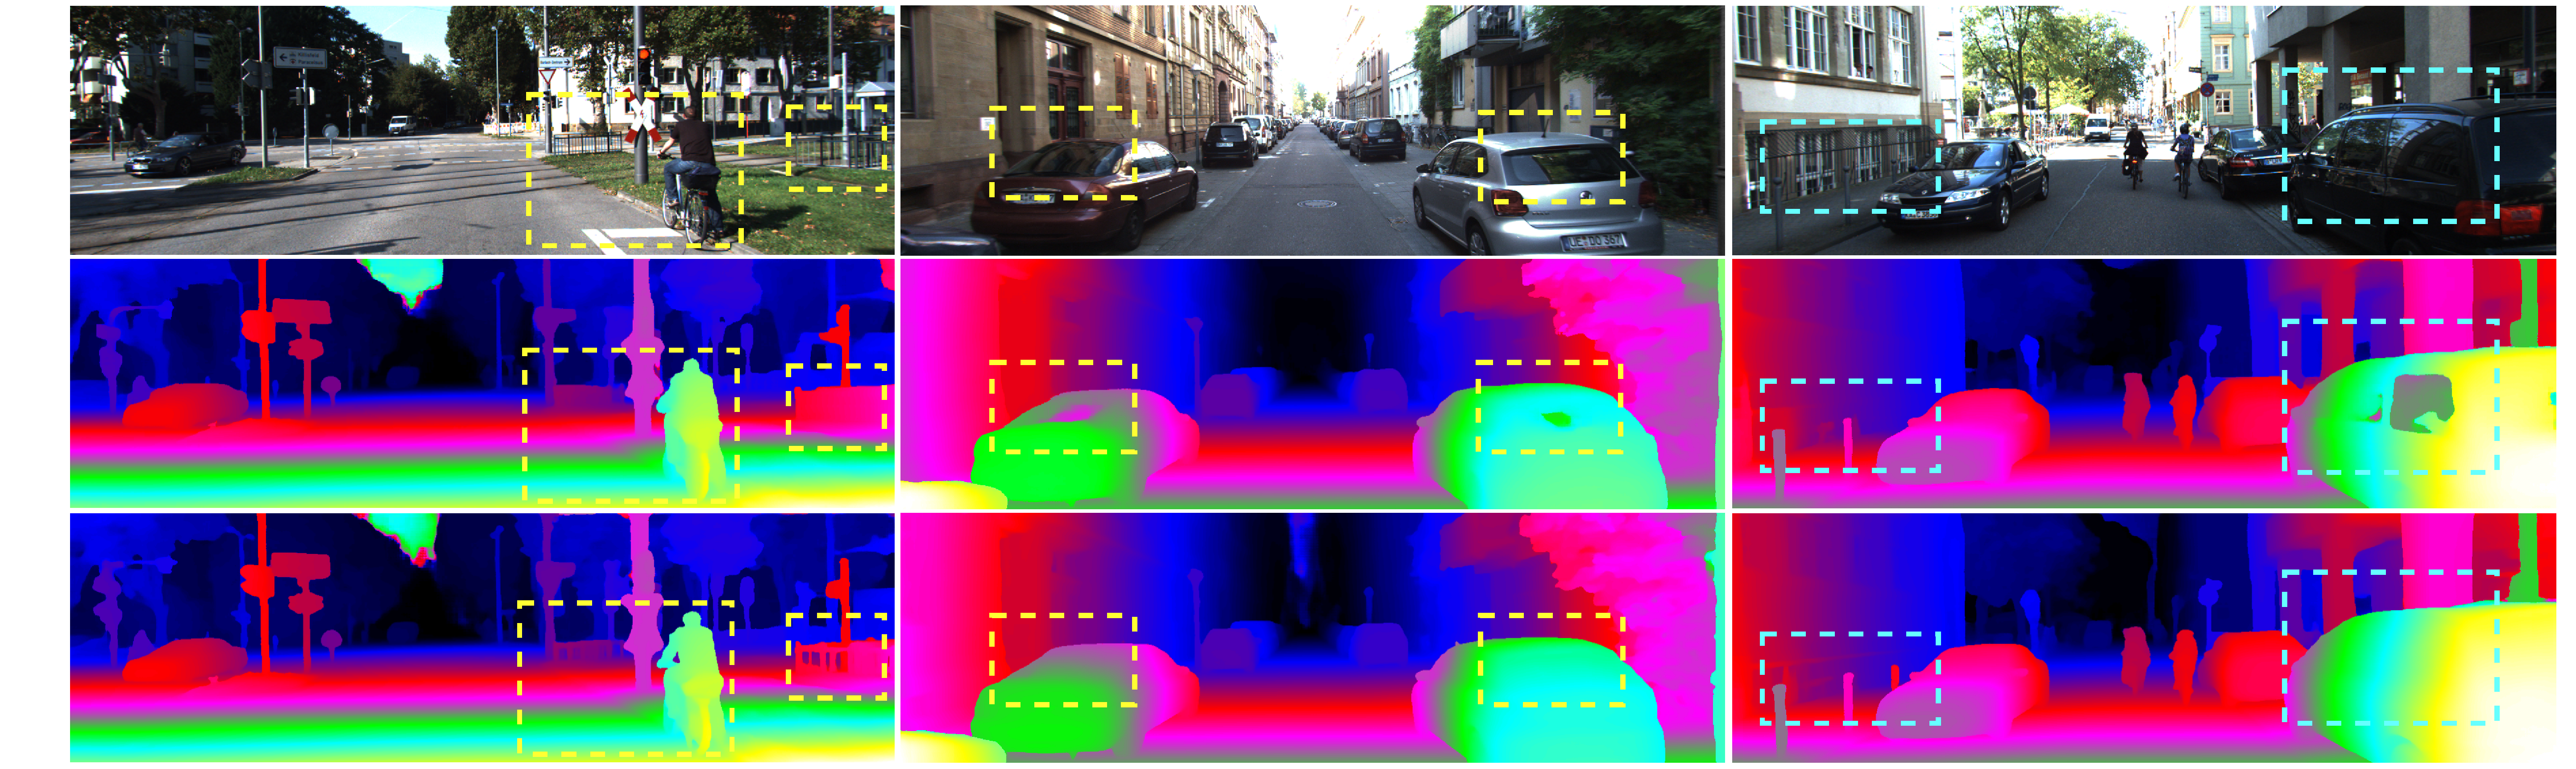
\includegraphics[width=0.96\linewidth]{fig/bridgedepth/kitti_ft.pdf} \\
	\end{tabular}
	\vspace{-0.5em}
	\caption{\textbf{Visual comparison on KITTI using a model fine-tuned on the combined KITTI 2012 and 2015 training sets}. 
	Relative to the state-of-the-art stereo method NMRF~\cite{guan2024neural}, the proposed approach better handles challenging regions such as transparent windows while maintaining fine structural detail.}
	\label{fig:kitti_ft}
	\vspace{-1.0em}
\end{figure}

\noindent\textbf{Zero-shot generalization.}
To evaluate cross-domain robustness, models trained only on Scene Flow are directly tested on real-world datasets without fine-tuning.
This setting is challenging for stereo matching because the appearance statistics, camera configurations, image noise, and disparity distributions differ significantly from the synthetic training domain.
The proposed stereo output improves substantially over the NMRF baseline on Middlebury and ETH3D.
The quantitative results are reported in Table~\ref{tab:bridge_zero_shot}. 
On Middlebury at quarter resolution, BP-2 error decreases from $7.5\%$ to $4.3\%$. On ETH3D, the BP-1 error decreases from $3.8\%$ to $1.3\%$.
The monocular output also generalizes well after alignment, indicating that stereo geometry improves the contextual branch rather than benefiting only the stereo prediction.
The substantial gains on ETH3D and Middlebury support the thesis argument that robust visual geometry benefits from combining complementary cues within a unified latent representation.

\begin{figure}[!t]
	\centering
	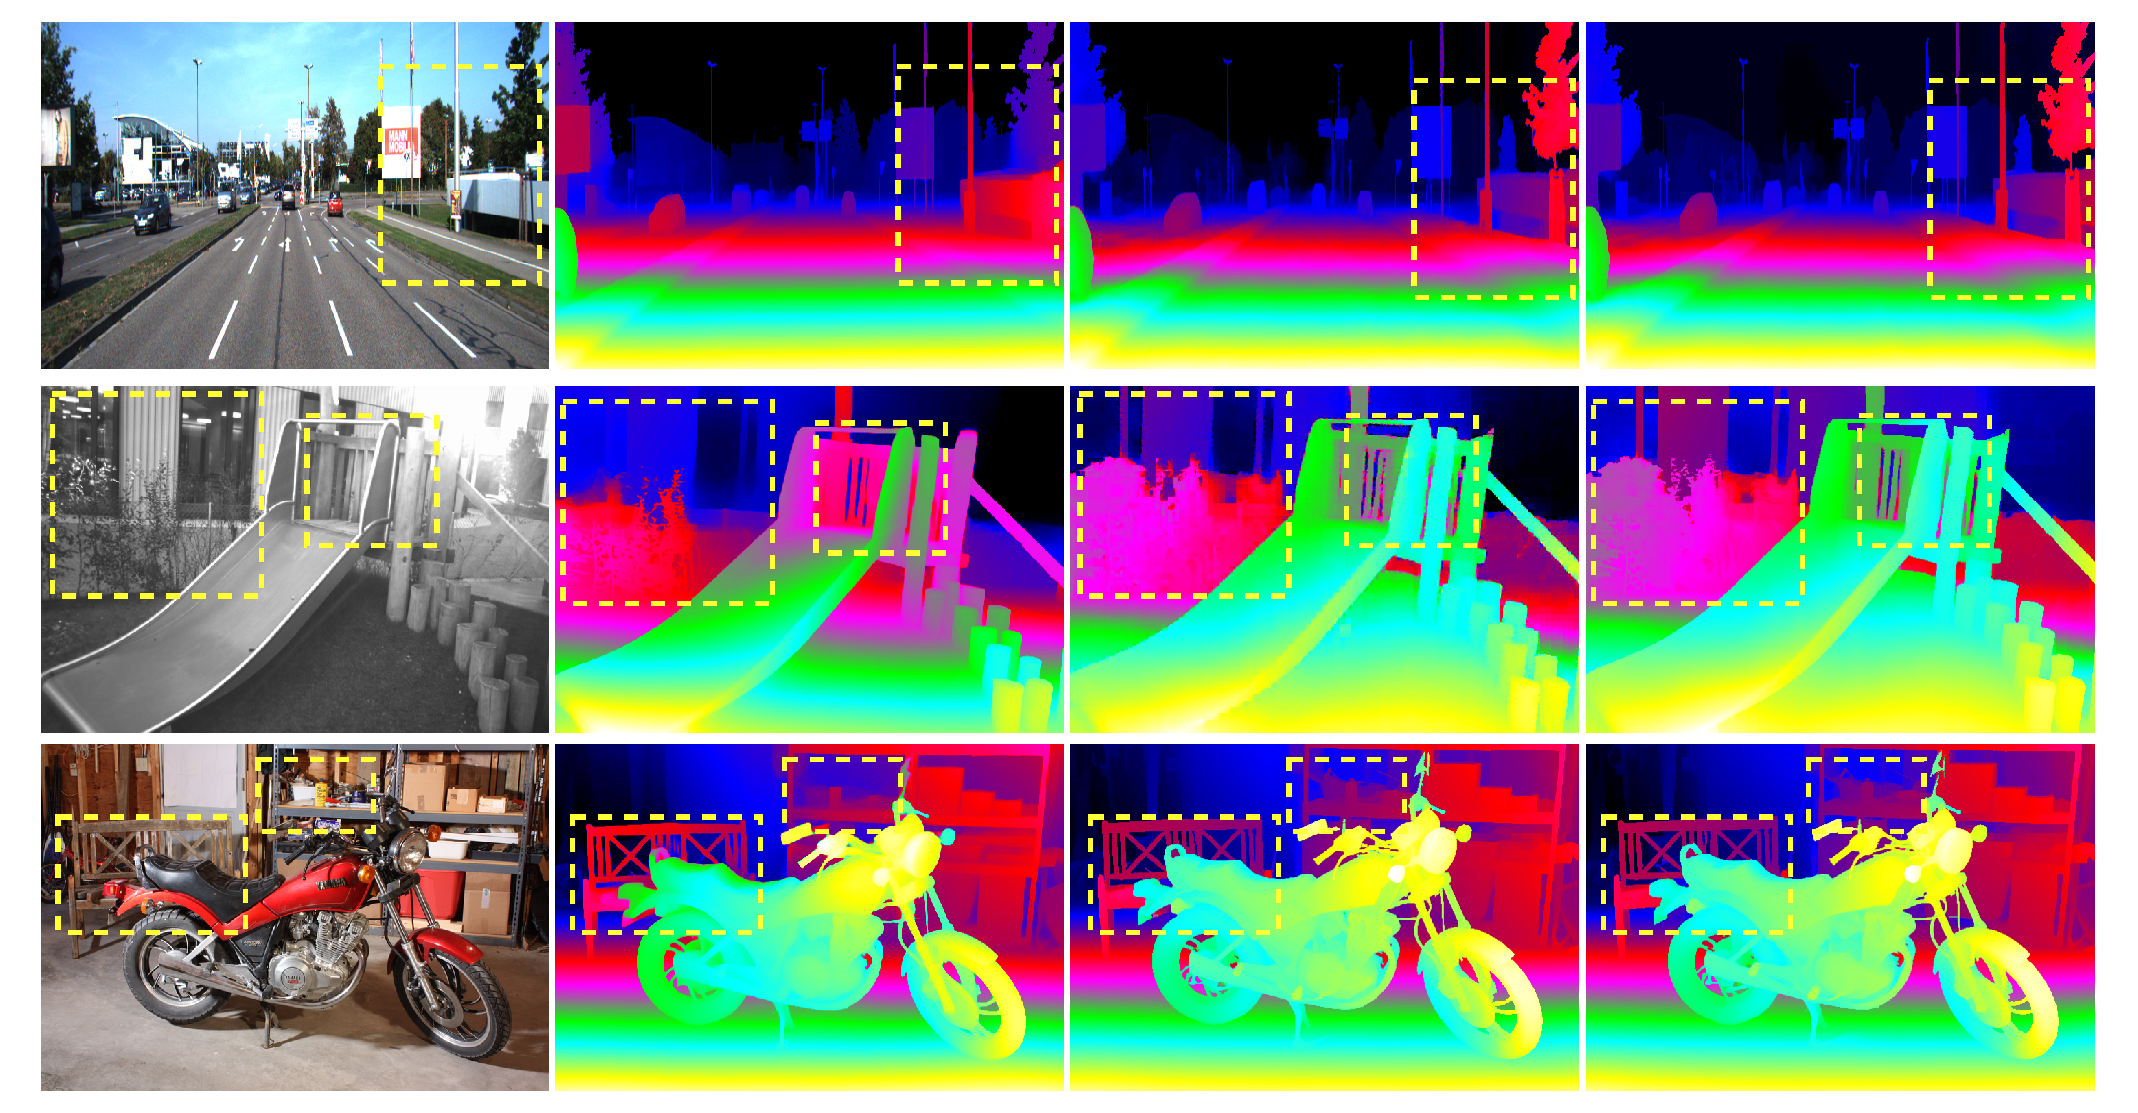
\includegraphics[width=1.0\linewidth]{fig/bridgedepth/zeroshot_mono.pdf}\\
	\vspace{-4pt}
	\makebox[0.245\linewidth]{\footnotesize\textsf{Input Image}}
	\makebox[0.24\linewidth]{\footnotesize\textsf{DAv2~\cite{yang2024depth}}}
	\makebox[0.24\linewidth]{\footnotesize\textsf{Ours-\emph{Mono}}}
	\makebox[0.245\linewidth]{\footnotesize\textsf{Ours-\emph{Stereo}}}\\
	\vspace{-4pt}
	\caption{\textbf{Zero-shot generalization of monocular depth outputs.} 
	Compared with DepthAnythingV2~\cite{yang2024depth}, the monocular stream of BridgeDepth produces estimates with stronger scale coherence and finer structural detail.}
	\label{fig:mono_zero}
	\vspace{-0.5em}
\end{figure}

\noindent\textbf{Ill-posed reflective and transparent regions.}
Qualitative evaluation on the Booster dataset, illustrated in Figure~\ref{fig:bridge_stereo_zero}, shows the benefit of latent alignment in regions where stereo correspondence is intrinsically ambiguous.
Matching-based stereo methods can produce fragmented predictions near mirrors, glass, transparent bottles, or specular hightlights because the apparent correspondence does not reliably represent the physical surface.
In contrast, the proposed method maintains more coherent surface structure by using monocular context to regularize stereo hypotheses.
This behavior is consistent with the design of the readout phase.
Stereo hypotheses query monocular features before aggregation, so the hypothesis representation has access to structural priors before selecting or propagating disparities.
As a result, the model is less likely to rely solely on local matching evidence in regions where that evidence is misleading.

\begin{figure}[!t]
	\centering
	\begin{minipage}{0.45\linewidth}
		\centering
		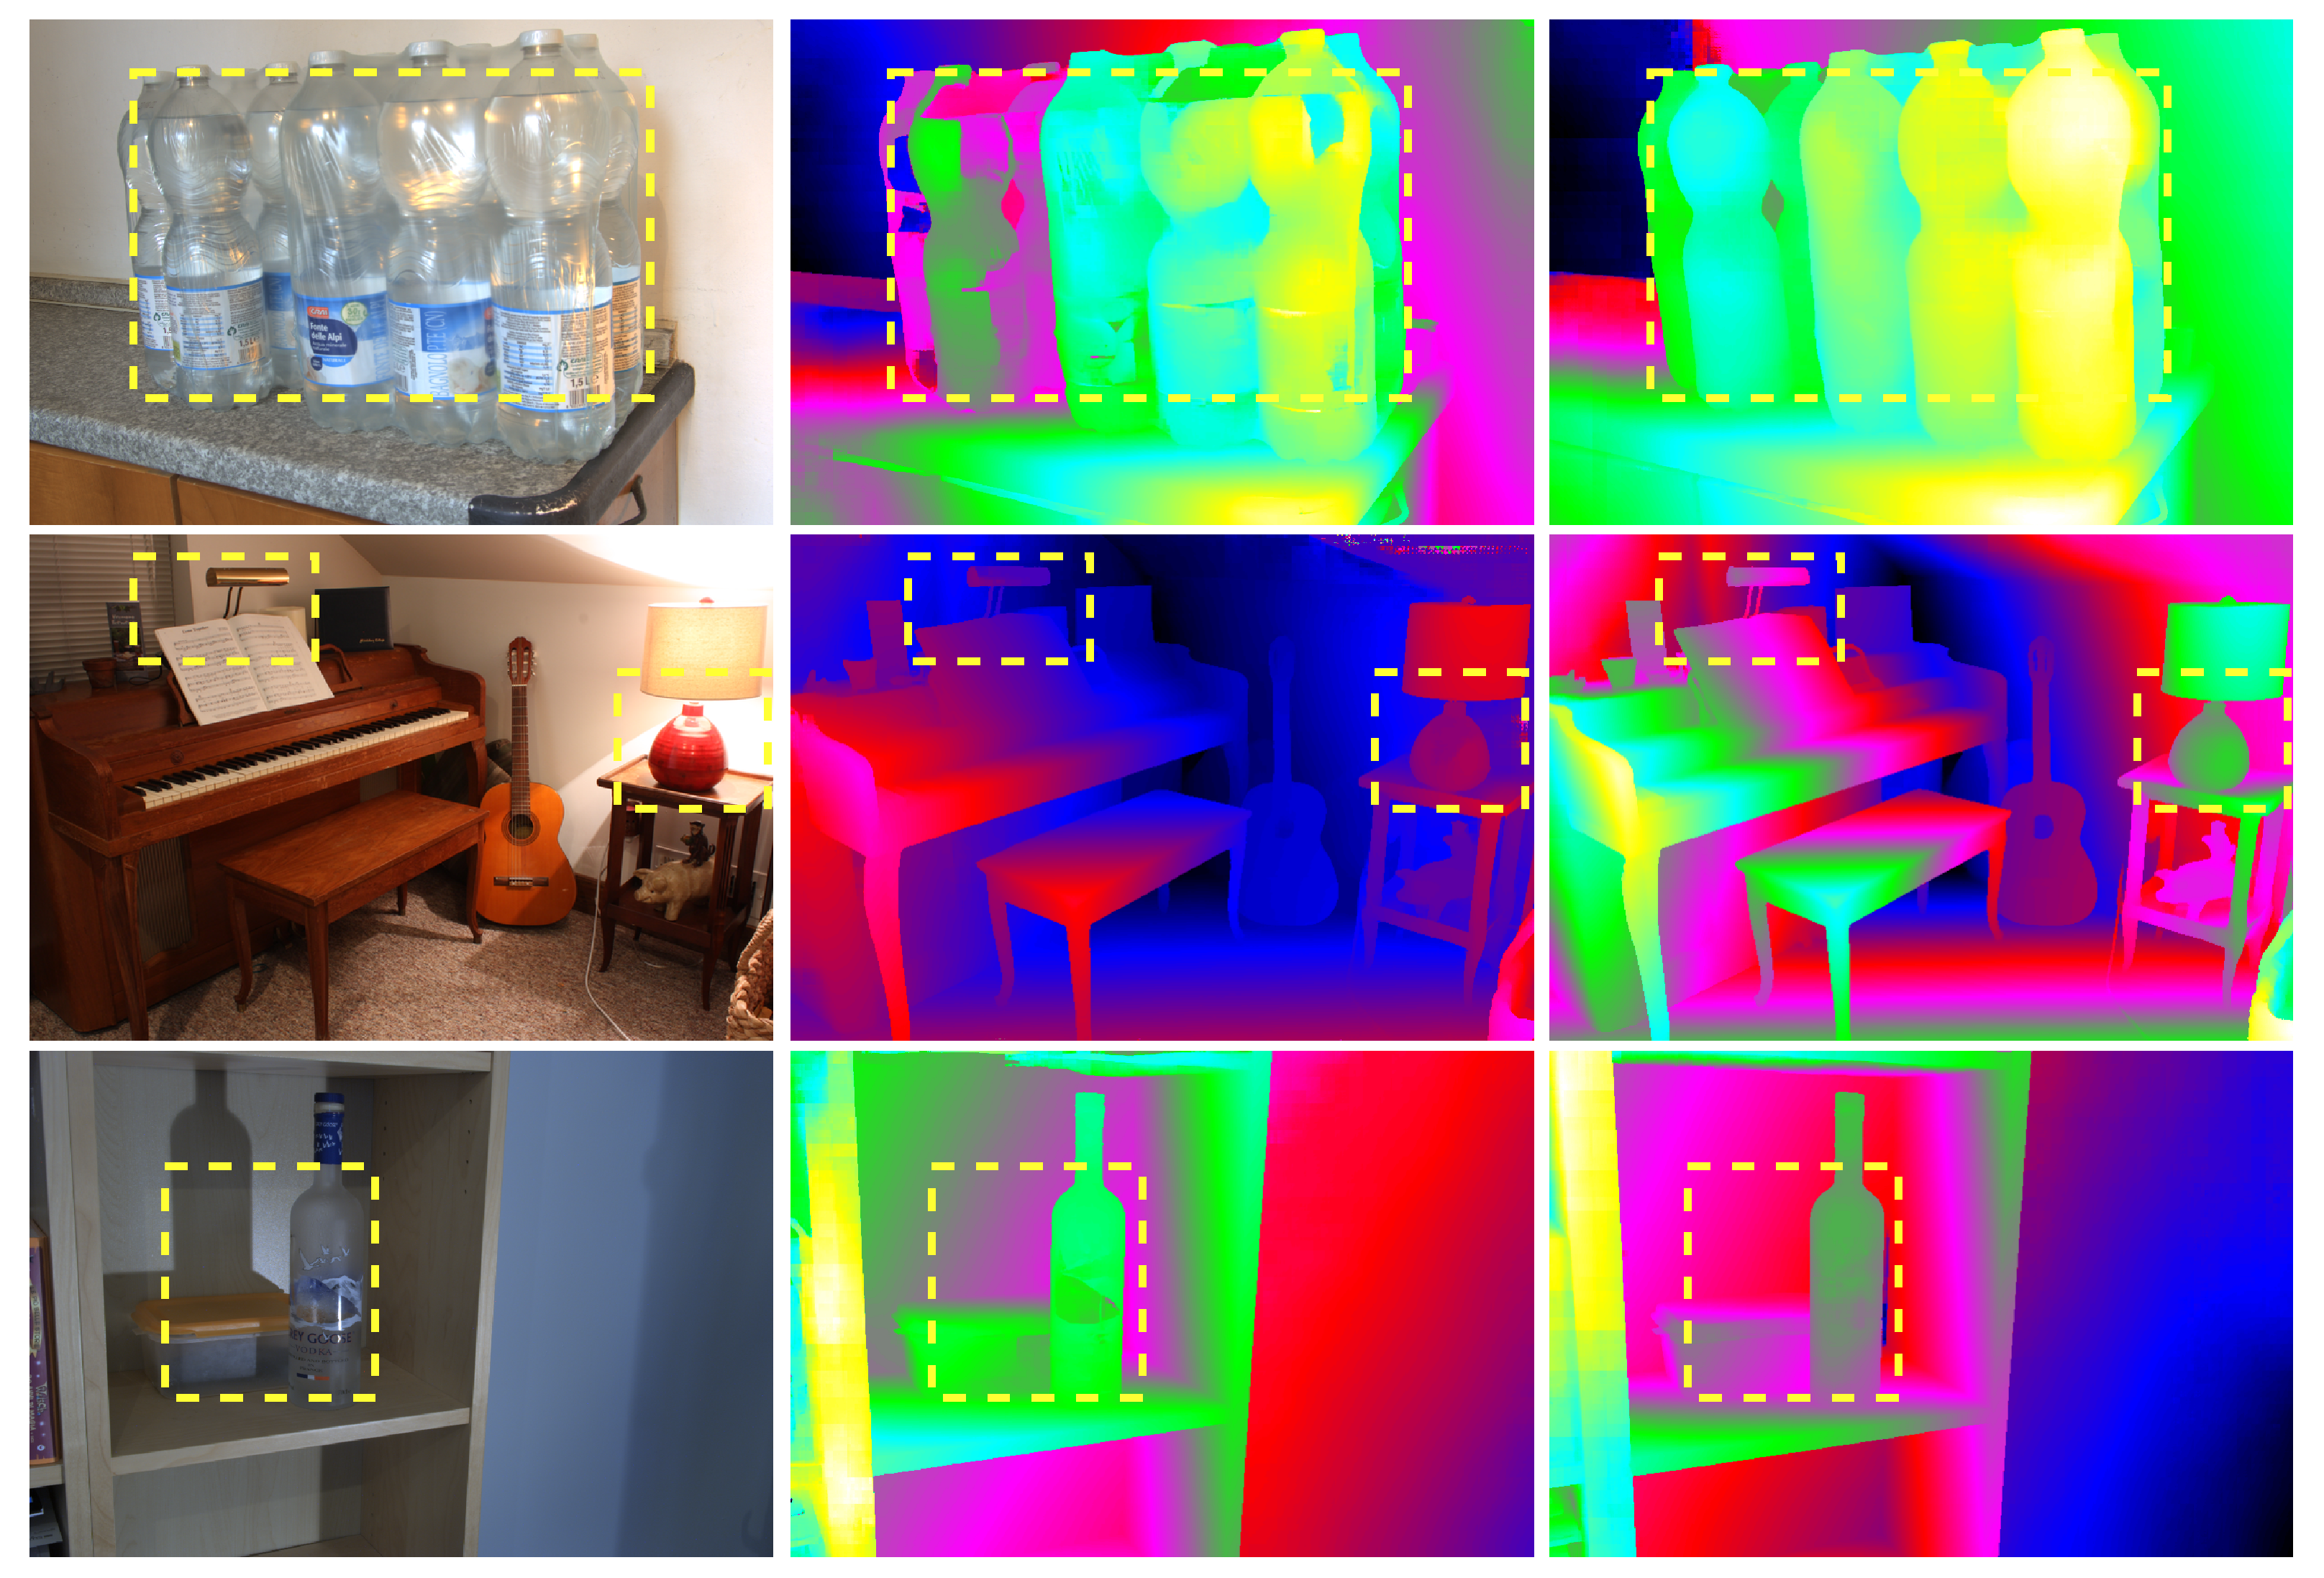
\includegraphics[width=\linewidth]{fig/bridgedepth/zero_stereo.pdf}
		\vspace{-3pt}
		\makebox[0.33\linewidth]{\footnotesize\textsf{Input Image}}
		\makebox[0.32\linewidth]{\footnotesize \textsf{NMRF}~\cite{guan2024neural}}
		\makebox[0.32\linewidth]{\footnotesize \textsf{Our-\emph{Stereo}}}
		%\subcaption{\textbf{Zero-shot stereo performance on ill-posed scenes.} Qualitative comparison between our method and the NMRF~\cite{guan2024neural} in difficult correspondence regions.}
		\captionof{figure}{\textbf{Zero-shot stereo performance on ill-posed scenes.}
		Qualitative comparison between the proposed method and NMRF~\cite{guan2024neural} in difficult correspondence regions.}
		\label{fig:bridge_stereo_zero}
	\end{minipage}
	\hfill
	\begin{minipage}{0.54\linewidth}
		\centering
		\resizebox{\linewidth}{!}{
		\begin{tabular}{l c c c c}
			\toprule
			\multirow{2}{*}{Methods} & KITTI-12 & KITTI-15 & Middlebury (Q) & ETH3D \\
			& (D1) & (D1) & (BP-2) & (BP-1) \\
			\midrule
			DSMNet~\cite{zhang2019domaininvariant} & 6.2 & 6.5 & 8.1 & 6.2\\
			Mask-CFNet~\cite{rao2023masked} & 4.8 & 5.8 & - & 5.7 \\
			
			CREStereo++~\cite{jing2023uncertainty} & 4.7 & 5.2 & - & 4.4\\
			Former-RAFT-DAM~\cite{zhang2024learning} & 3.9 & 5.1 & 5.4 & 3.3 \\
			RAFT-Stereo~\cite{lipson2021raft} & 4.7 & 5.5 & 9.4 & 3.3\\
			
			IGEV-Stereo~\cite{xu2023iterative} &5.2 & 5.7 & 8.8 & 4.0\\
			NMRF~\cite{guan2024neural} & 4.2 & 5.1 & 7.5 & 3.8\\
			IGEV++~\cite{xu2024igev++} & 5.1 & 5.9 & 7.8 & 4.1 \\
			FoundationStereo~\cite{wen2025foundationstereo} & \cellcolor{red!25}\textbf{3.2} & \cellcolor{yellow!25}4.9 & \cellcolor{yellow!25}5.5 & \cellcolor{yellow!25}1.8 \\
			\midrule
			BridgeDepth (Stereo) & \cellcolor{yellow!25}3.6 & \cellcolor{red!25}\textbf{4.5} & \cellcolor{red!25}\textbf{4.3} & \cellcolor{red!25}\textbf{1.3}\\
			BridgeDepth (Mono$^\dag$) & 3.7 & 4.2 & 5.8 & 1.7\\
			\bottomrule
		\end{tabular}
		}
		\captionof{table}{\textbf{Evaluation under zero-shot generalization.} All methods are trained exclusively on the Scene Flow dataset. The \colorbox{red!25}{\textbf{best}} and \colorbox{yellow!25}{second best} are color-coded. ($\dag$): Relative depth maps are aligned to ground truth using the ROE solver~\cite{wang2025moge}.}
		\label{tab:bridge_zero_shot}
	\end{minipage}
	%\vspace{-1.0em}
	%\caption{Left: Qualitative comparison on ill-posed stereo regions. Right: Quantitative zero-shot benchmarks for all methods trained solely on Scene Flow.}
\end{figure}

\noindent\textbf{ETH3D leaderboard evaluation.} On the ETH3D test set, the method also achieves state-of-the-art performance compared with recent stereo and hybrid systems.
As reported in Table~\ref{supp:tab_eth3d}, the method obtains $0.50\%$ BP-1 error, $0.16\%$ BP-2 error, $0.11$ pixel average error, and $0.26$ pixel RMS error.
These results demonstrate that our approach delivers accurate and robust depth estimation across diverse real-world conditions.

\begin{table}[!t]
	\centering
	\begin{subtable}{0.49\linewidth}
			%\vspace{0.2em}
			\footnotesize
			%\setlength\tabcolsep{2.5pt}
			%\renewcommand{\thetable}{{\alph{table}}}
			\centering
			\begin{tabular}{c|cccc}
				\toprule
				Method & BP-1 & BP-2 & AvgErr & RMS \\
				\midrule
				LoS~\cite{li2024local} & 1.03 & 0.32 & 0.15 & 0.34\\
				IGEV++~\cite{xu2024igev++} & 1.58 & 0.76 & 0.19 & 0.74\\
				Selective-IGEV~\cite{wang2024selective} & 1.56 & 0.51 & 0.15 & 0.57\\
				DEFOM-Stereo~\cite{jiang2025defom} & 0.78 & \underline{0.19} & \textbf{0.11} & \textbf{0.26}\\
				FoundationStereo~\cite{wen2025foundationstereo} & \textbf{0.48} & 0.26 & 0.13 & 0.61\\
				BridgeDepth (Ours) & \underline{0.50} & \textbf{0.16} & \textbf{0.11} & \textbf{0.26}\\
				\bottomrule
			\end{tabular}
			\caption{Performance on ETH3D test split}
			\label{supp:tab_eth3d}
	\end{subtable}
	\hfill
	\begin{subtable}{0.49\linewidth}
		\footnotesize
		\begin{tabular}{l c c c}
			\toprule
			& ETH3D & Middlebury & Time \\
			& (BP-1) & (BP-2) & (s) \\
			\midrule
			baseline (NMRF-s) & 3.7 & 8.0 & 0.044\\
			w/ monocular-readout & 2.3 & 5.9 & 0.123\\
			w/ monocular-update & 2.1 & 5.5 & 0.128\\
			w/ fine-grained & 1.6 & 4.8 & 0.147\\
			w/ monocular loss & 1.3 & 4.4 & 0.147\\
			\bottomrule
		\end{tabular}
		\caption{Impact assessment of individual architecture modules.}
		\label{tab:bridge_abl}
	\end{subtable}
	\vspace{-1.0em}
	\caption{Quantitative assessment of the proposed framework. Subtable (a) reports accuracy metrics on the ETH3D test set. Subtable (b) isolates the contribution of each architectural module through ablation.}
\end{table}

\noindent\textbf{Monocular output evaluation.} To evaluate the monocular stream, its relative depth prediction is aligned to the ground-truth disparity before computing the metrics.
Specifically, relative depth maps are aligned to ground truth using the ROE solver~\cite{wang2025moge}.
Compared with the original monocular foundation model and representative monocular metric depth models, the aligned monocular output achieves substantial improvement in Abs Rel and $\delta < 1.25$ across KITTI, ETH3D, and Middlebury, as shown in Table~\ref{supp:tab_depth}.
These results suggest that the monocular stream is not merely  a source of contextual priors for stereo matching.
Through bidirectional update, its latent representation is progressively grounded by aggregated stereo hypotheses and becomes more consistent with metric multi-view geometry.
This further verifies that BridgeDepth establishes mutual refinement between monocular context and stereo correspondence, rather than using monocular priors only as one-way guidance for stereo matching.

\begin{table}[t]
	%\vspace{-1em}
	\footnotesize
	\centering
	\begin{tabular}{c|cc|cc|cc|cc}
		\toprule
		\multirow{2}{*}{Model}& \multicolumn{2}{c|}{KITTI-12} & \multicolumn{2}{c|}{KITTI-15} & \multicolumn{2}{c|}{ETH3D} & \multicolumn{2}{c}{Middlebury}\\
		& Abs Rel $\downarrow$ & $\delta<1.25 \uparrow$ & Abs Rel $\downarrow$ & $\delta<1.25 \uparrow$ & Abs Rel $\downarrow$ & $\delta<1.25 \uparrow$ & Abs Rel $\downarrow$ & $\delta<1.25 \uparrow$ \\
		\midrule
		DAv2-L & 0.093 & 0.925 & 0.084 & 0.933 & 0.055 & 0.965 & 0.081 & 0.943\\
		UDv2-L & 0.054 & 0.967 & 0.067 & 0.949 & 0.052 & 0.972 & 0.056 & 0.982\\
		Ours & \textbf{0.033} & \textbf{0.982} & \textbf{0.048} & \textbf{0.975} & \textbf{0.020} & \textbf{1.000} & \textbf{0.019} & \textbf{0.990}\\
		\bottomrule
	\end{tabular}
	\vspace{-1.0em}
	\caption{\textbf{Monocular output evaluation.}
	Relative depth predictions are aligned to the ground-truth disparity using the ROE solver of MoGe~\cite{wang2025moge}.
	DAv2-L denotes the ViT-L variant of DepthAnythingV2, and UDv2-L denotes the ViT-L variant of UniDepthV2~\cite{piccinelli2025unidepthv2}.
	The monocular output of BridgeDepth achieves substantial improvement across KITTI, ETH3D, and Middlebury.
	}
	\label{supp:tab_depth}
	\vspace{-1.2em}
\end{table}

\subsection{Ablation Studies}
The ablation studies clarify how each component contributes to the central objective of this chapter: aligning monocular contextual reasoning with stereo hypothesis-based geometry.
Rather than treating the results only as incremental numeric improvements, the analysis focuses on three questions.
First, does the monocular stream provide useful structural priors for stereo matching under domain shift?
Second, does the reverse update from stereo to monocular representation contribute to genuine bidirectional alignment rather than one-way guidance?
Third, can the model recover fine geometric details without sacrificing the efficiency gained from compact stereo hypotheses?

All variants in Table~\ref{tab:bridge_abl} are trained only on Scene Flow and evaluated in the zero-shot setting on ETH3D and Middlebury.
This setting is intentionally chosen because it stresses the generalization ability of stereo matching.
A model trained only on synthetic data must handle real image statistics, different camera settings, grayscale imagery, and challenging regions where local correspondence evidence is often unreliable.
Improvement in this setting is therefore more informative than in-domain accuracy alone: it indicates whether the model has learned a more transferable form of geometric reasoning.
The baseline is a streamlined stereo-only model derived from NMRF~\cite{guan2024neural}.
It keeps the core hypothesis-based stereo formulation, including compact disparity proposals and neural message passing, but removes the monocular branch and all cross-modal alignment operations.
To make the comparison controlled and efficient, the baseline uses only two disparity hypotheses per pixel, matching the compact hypothesis representation used by BridgeDepth.
In this way, the baseline isolates the capability of stereo hypothesis reasoning alone.
Its performance reflects the limitation of relying only on binocular evidence when the candidate disparity set is small and the test domain differs from the training domain.

\noindent\textbf{Monocular readout.} As shown in Table~\ref{tab:bridge_abl}, adding monocular readout brings the most significant improvement.
In this variant, stereo hypotheses query monocular contextual representations before neural message passing.
This result confirms the primary motivation of this chapter: monocular representations are more useful when they participate in stereo reasoning before the model aggregates and selects hypotheses.
Since readout is applied before cost aggregation, contextual cues about scene layout, object structure, and surface continuity can guide how ambiguous hypotheses are propagated and suppressed.
The substantial improvement on ETH3D, where BP-1 decreases from 3.7\% to 2.3\%, and on Middlebury, where BP-2 decreases from 8.0\% to 5.9\%, suggests that monocular priors help compensate for unreliable correspondence evidence under domain shift.

\noindent\textbf{Monocular update.} The monocular update module completes the bidirectional alignment loop. 
Compared with monocular readout alone, the gain in stereo metrics is moderate, which is expected because the update primarily refines the monocular representation rather than directly changing the current stereo hypotheses.
Its value lies in the iterative nature of the model: once the monocular stream has absorbed aggregated stereo evidence, the updated contextual representation can provide more geometry-aware guidance in subsequent alignment blocks.
Therefore, the update step should not be interpreted only by its immediate numeric improvement in the stereo output.
It is important because it changes the role of the monocular stream from a fixed source of priors into a geometry-grounded representation that participates in mutual refinement.

\noindent\textbf{Fine-grained refinement.} The fine-grained refinement stage addresses a different limitation of the coarse alignment process.
The main bidirectional alignment operates at $1/8$ resolution for efficiency, which is suitable for robust global reasoning but insufficient for thin structures, sharp boundaries, and small disparity variations.
The fine stage initializes high-resolution stereo embeddings from the coarse prediction and performs additional alignment at $1/4$ resolution.
Importantly, the monocular stream remains at the coarse resolution, and the interaction window is adjusted to preserve a comparable receptive field.
This asymmetric design improves detail recovery while avoiding the high computational cost of full high-resolution cross-modal alignment.
The ablation therefore shows that fine-scale stereo evidence and coarse contextual priors can be combined efficiently.

\noindent\textbf{Monocular loss.} Finally, adding the monocular loss produces the strongest generalization performance.
This loss does not merely provide auxiliary supervision to an additional output.
It explicitly encourages the monocular representation to remain consistent with ground-truth geometry after receiving stereo updates.
As a result, bidirectional alignment is strengthened from both directions: stereo hypotheses are guided by monocular context, and monocular representations are encouraged to encode geometry consistent with stereo disparity.
The qualitative comparison in Figure~\ref{fig:abl} further supports this interpretation, showing that monocular supervision improves the structural consistency of the aligned representation and reduce artifacts in ambiguous regions.

\begin{figure}[!t]
	\centering
	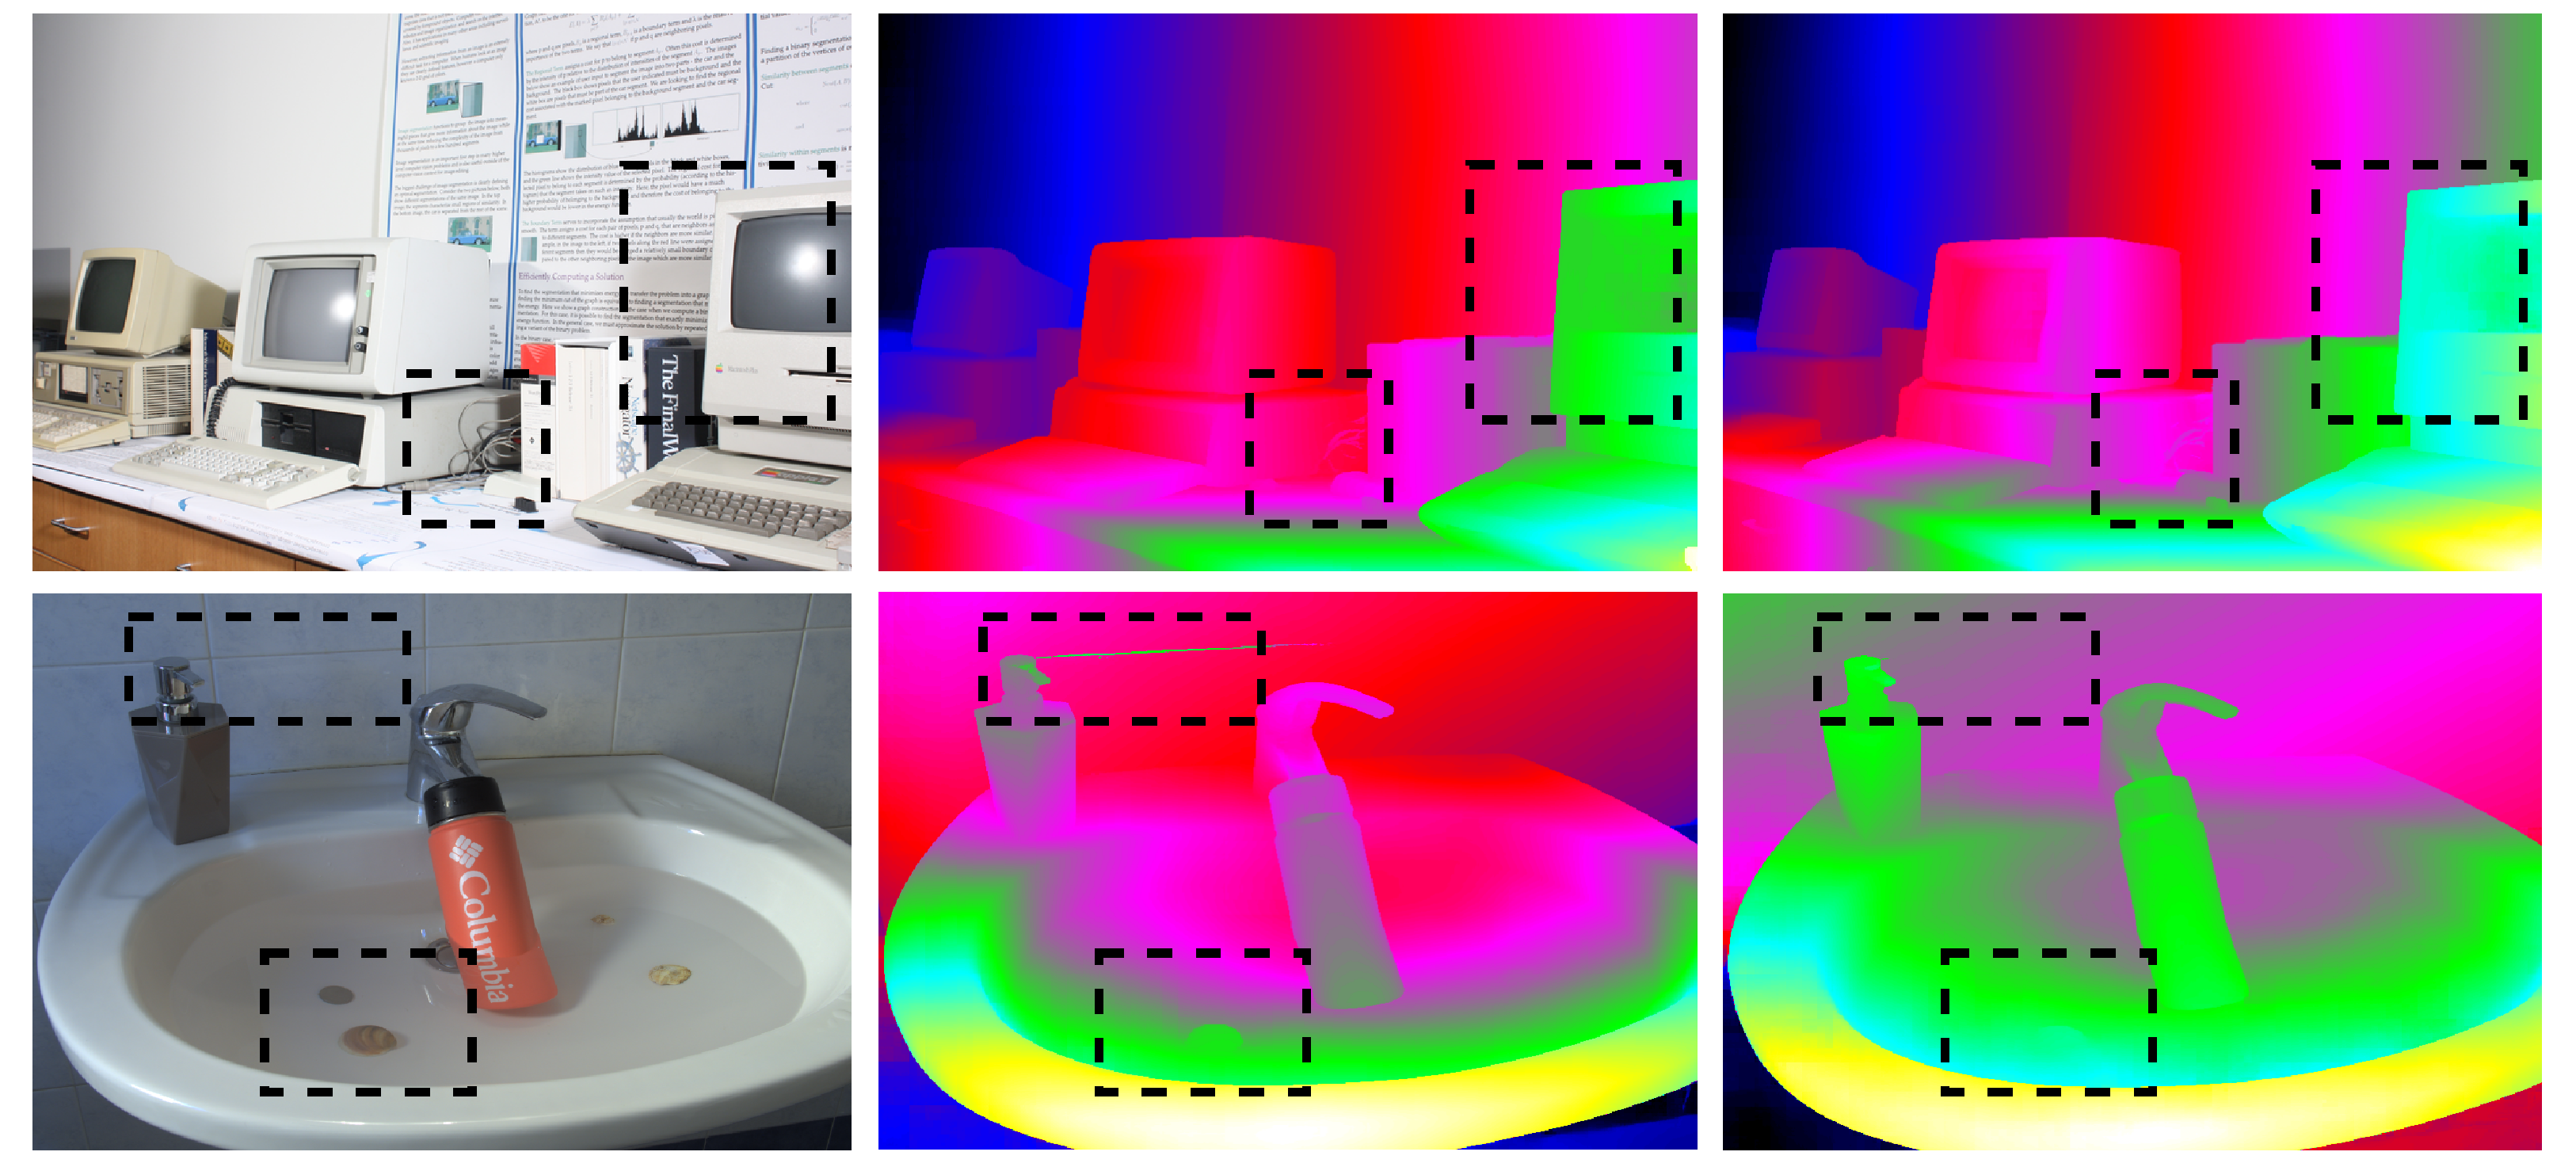
\includegraphics[width=0.75\linewidth]{fig/bridgedepth/abl.pdf}\\
		\vspace{-4pt}
		\makebox[0.25\linewidth]{\footnotesize\textsf{Input Image}}
		\makebox[0.24\linewidth]{\footnotesize $\mathcal{L}_{\text{stereo}}$}
		\makebox[0.25\linewidth]{\footnotesize$\mathcal{L}_{\text{stereo}}+\mathcal{L}_{\text{mono}}$}\\
		%\includegraphics[width=0.97\linewidth]{figs/zero-shot-booster.pdf}
		\vspace{-0.3em}
		\captionof{figure}{\textbf{Effect of monocular supervision.}
		Adding the monocular loss improves the geometric consistency of the aligned representation, producing more coherent depth structures in ambiguous regions than stereo-only supervision.}
		\label{fig:abl}
\end{figure}

\begin{table}[!t]
	\centering
	\footnotesize
	\begin{tabular}{c|c|cccc}
		\toprule
		\multirow{2}{*}{Backbone} & SceneFlow & KITTI-12 & KITTI-15 & ETH3D & Middlebury (Q)\\
		& EPE $\downarrow$ & D1 $\downarrow$ & D1 $\downarrow$ & BP-1 $\downarrow$ & BP-2 $\downarrow$\\
		\midrule
		baseline & 0.47 & 4.5 & 5.2 & 3.7 & 8.0\\
		\rowcolor{lightgray}
		DAv2-B & 0.37 & 3.8 & 4.7 & 1.4 & 4.7\\
		DAv2-L & 0.37 & 3.7 & 4.5 & 1.3 & 4.4\\
		UDv2 & 0.36 & 3.7 & 4.8 & 1.8 & 5.1\\
		MoGe & 0.36 & 3.3 & 4.5 & 1.8 & 5.1\\
		\midrule
		\rowcolor{lightgray}
		DAv2-B (post-hoc)&0.44&4.1&4.8&3.2&7.4\\
		\bottomrule
	\end{tabular}
	\vspace{-0.3em}
	\captionof{table}{\textbf{Ablation of monocular foundation models and fusion strategy.}
	We report in-domain accuracy on Scene Flow and zero-shot generalization on real-world datasets.
	The baseline is the NMRF model used in Table~\ref{tab:bridge_abl}.
	Here, DAv2 denotes DepthAnythingV2, and UDv2 denotes UniDepthV2.
	The gray rows use the same DAv2-B backbone to compare latent alignment with post-hoc fusion, showing that interaction during hypothesis reasoning is more effective than late-stage fusion.
	}
	\label{tab:mono_foundation}
	\vspace{-1.0em}
\end{table}

\noindent\textbf{Monocular foundation models and post-hoc fusion.} 
Beyond the main component analysis in Table~\ref{tab:bridge_abl}, additional ablations examine whether the proposed mechanism depends on a particular monocular foundation model and whether iterative alignment is preferable to post-hoc fusion. 
Replacing the monocular backbone with different foundation models still yields clear improvements over the stereo-only baseline, as shown in Table~\ref{tab:mono_foundation}).
This indicates that the framework is not tied to one specific monocular architecture.
Although the backbone affects final accuracy to some extent, the consistent trend suggests that the benefit comes from the alignment mechanism itself: stereo hypotheses can exploit high-level monocular structure as long as the monocular branch provides meaningful contextual features.

The post-hoc fusion ablation further clarifies this point.
In that variant, monocular features are fused with the already aggregated stereo representation using a lightweight residual network, bypassing the iterative readout-update process.
Although this static fusion introduces additional monocular context, it performs noticeably worse than bidirectional latent alignment, as shown in Table~\ref{tab:mono_foundation}).
This comparison is important for the thesis argument.
It shows that the gain does not simply come from adding a monocular stream or increasing model capacity.
The crucial factor is when and how the modalities interact.
If the modalities are fused only after most reasoning has already been completed, monocular context cannot effectively guide hypothesis selection, and stereo geometry cannot progressively ground the monocular representation.
Dynamic alignment during inference is therefore essential for learning a unified geometric representation.

Overall, the ablation studies support the design principle of BridgeDepth.
The stereo-only baseline demonstrates the limitation of matching-centric reasoning in ambiguous regions.
Monocular readout shows that contextual priors are most effective when introduced before stereo aggregation.
Monocular update and monocular supervision demonstrate that the monocular stream can be made geometry-aware rather than remaining a fixed prior.
Fine-grained refinement shows that local detail can be recovered without abandoning the efficient coarse alignment design.
Together, these results validate the central claim of this chapter: robust depth estimation benefits from a shared latent space in which monocular context and stereo correspondence are repeatedly exchanged and refined.

\section{Discussion}
\subsection{Why Latent Alignment Improves Generalization}
The improvement in zero-shot generalization can be understood from the different failure modes of monocular and stereo estimation.
Stereo matching depends on local correspondence evidence and therefore suffers when the target domain changes appearance statistics or contains ambiguous surfaces.
Monocular foundation models, trained on diverse data, encode more domain-robust priors about object shape and scene layout.
By allowing stereo hypotheses to read from monocular features during aggregation, the model can use these priors to regularize matching in unfamiliar domains.
At the same time, monocular prediction lacks metric grounding.
The update operation addresses this limitation by injecting aggregated stereo evidence into the monocular stream.
The resulting monocular representation is not merely a prior learned from single images; it becomes conditioned on multi-view geometry.
This mutual refinement explains why both outputs improve.

\subsection{Relation to the Thesis Narrative}
This chapter fits into the broader thesis theme of learning visual geometry by unifying complementary cues.
Stereo correspondence provides spatial geometry through multi-view constraints, while monocular depth estimation provides semantic and structural priors.
Neither cue is sufficient in isolation.
Stereo is precise but fragile under ambiguity; monocular reasoning is robust but geometrically under-constrained.
The latent alignment framework shows how a neural network can explicitly coordinate these cues in representation space.
The same principle extends naturally to temporal geometry.
Optical flow and camera motion provide another source of geometric information, but they also suffer from ambiguity, occlusion, and appearance changes.
A future geometry-native architecture could similarly align temporal correspondence representation with monocular structural priors.
Thus, the contribution of this chapter is not only a stereo depth estimator, but also a concrete example of the thesis hypothesis: robust depth and motion perception requires unified representations that allow different geometric cues to interact during inference.

\subsection{Limitations}
Although the proposed framework improves robustness and generalization, it still has limitations.
First, the use of a top-$K$ disparity proposal module may become restrictive at very high image resolutions or under very large disparity ranges.
If the correct disparity is not retained among the selected candidates, later alignment cannot recover it.
This issue can become more pronounced for images above 2K or scenes with a large disparity range.
Second, the monocular stream introduces additional computation and memory compared with a purely stereo network.
Although the proposed approach remains highly efficient relative to many concurrent hybrid systems, the cost of using a large monocular foundation model is non-negligible.

\section{Conclusion}
This chapter presented a latent alignment framework for bridging monocular contextual reasoning and stereo geometric matching.
The proposed model represents stereo matching as a compact set of disparity hypotheses and aligns these hypotheses with monocular foundation representations through iterative bidirectional cross-attention.
Monocular readout injects semantic and structural priors into stereo aggregation, while monocular update feeds geometrically validated stereo evidence back into the contextual representation. 
A coarse-to-fine refinement stage recovers local details, and a dual-output training objective jointly supervises metric disparity and relative depth.
Extensive experiments demonstrate that the framework improves both in-domain stereo accuracy and zero-shot generalization. 
It is especially effective in challenging regions where pure stereo matching is unreliable, such as reflective and transparent surfaces. 
Ablation studies confirm that dynamic latent alignment outperforms post-hoc fusion and that dual loss strengthens cross-modal consistency.

Within the thesis, this chapter provides an important step toward unified visual geometry learning.
It shows that monocular priors and stereo correspondences should not be treated as isolated modules, but as complementary cues that can be aligned and refined within a shared latent space.
This principle motivates the broader pursuit of depth and motion perception systems that integrate spatial, semantic, and temporal geometry in a coherent learning framework.